% !TEX encoding = UTF-8 Unicode
\documentclass{article}

\usepackage{amsmath}
\usepackage{mathtools}
\usepackage{graphicx, color}
\graphicspath{{figs/}}
\usepackage{natbib}
\usepackage{hyperref}
\usepackage{setspace}

%----------------------------------
%\topmargin      -1.5cm   % read Lamport p.163
%\oddsidemargin  -0.04cm  % read Lamport p.163
%\evensidemargin -0.04cm  % same as oddsidemargin but for left-hand pages
%\textwidth      16.59cm
%\textheight     22.94cm

\topmargin      -1.5cm   % read Lamport p.163
\oddsidemargin  -0.5cm  % read Lamport p.163
\evensidemargin -0.5cm  % same as oddsidemargin but for left-hand pages
\textwidth      16cm
\textheight     22.94cm

\parskip         7.2pt   % sets spacing between paragraphs
\parindent         3mm   % sets leading space for paragraphs

\setcounter{topnumber}{2}
\setcounter{bottomnumber}{2}
\setcounter{totalnumber}{4}
\renewcommand{\topfraction}{0.85}
\renewcommand{\bottomfraction}{0.85}
\renewcommand{\textfraction}{0.15}
\renewcommand{\floatpagefraction}{0.7}

\bibpunct{(}{)}{;}{a}{}{,} 

%-------------------------------------

\title{Bayesian Inference for  Covariance Matrix}
\author{Ignacio Alvarez}
\date{ Spring 2014 }

\begin{document}
 \pagenumbering{gobble}
 
\maketitle 


\begin{abstract}
Covariance matrix estimation arises in multivariate problems including multivariate normal sampling models and regression models where random effects are jointly modeled, e.g. random-intercept, random-slope models. A Bayesian analysis of these problems requires a prior on the covariance matrix. Here we assess, through a simulation study and a real data set, the impact this prior choice has on posterior inference of the covariance matrix.

Inverse Wishart distribution is the natural choice for a covariance matrix prior because its conjugacy on normal model and simplicity, is usually available in Bayesian statistical software. However inverse Wishart distribution presents some undesirable properties from a modeling point of view. It can be too restrictive because assume the same amount of prior information about every variance parameters and, more important, it shows a prior relationship between the variances and correlations.

Some alternatives distributions has been proposed. The scaled inverse Wishart distribution, which give more flexibility on the variance priors conserving the conjugacy property but does not eliminate the prior relationship between variances and correlations. Secondly, it is possible to fit separate priors for individual correlations and standard deviations. This strategy eliminates any prior relationship within the covariance matrix parameters, but it is not conjugate and therefore computationally slow. 
\end{abstract}

\newpage 
\tableofcontents

\newpage 
%\doublespacing
\pagenumbering{arabic} 

\section{Introduction} 

The estimation of a covariance matrix appears on multivariate problems and most commonly in the hierarchical model context. The inclusion of random effects in a linear model within Bayesian framework may lead to modeling the covariance matrix for those effects. Also regression models with varying coefficients across groups is one of the most common situation where a prior for a covariance matrix is needed. 

Bayesian estimation of a covariance matrix is a difficult problem, mainly because the standard approaches of conjugacy or non-informativeness present problems. In particular Jeffrey covariance prior may lead to improper posterior distributions when it is used in hierarchical models.  

The natural conjugate prior for the multivariate normal distribution is the inverse Wishart distribution. Conjugacy property has made of this choice the most commonly used approach for covariance matrix. However, this prior presents some problems, It can be too restrictive because assume the same amount of prior information about every variance parameters. More important, it shows a prior relationship between the variances and correlations, these characteristic of the prior can impact on posterior inferences about the covariance matrix. We show in this paper that even for simple models inverse Wishart prior may become an extremely informative prior resulting in biased inference for correlation and variances. In a scenario with small variability, inverse Wishart might severely underestimate the correlation and overestimate variances. 

There are many alternative ways to construct priors for the covariance matrices that have been proposed,  however \cite{visualize} states that 
 \textit{``even fewer analytical results are known for these families, making it even more challenging to understand precisely the properties of such distributions. Consequently, our analytical understanding of these distributions falls short of providing us a full understanding of the inverse-Wishart distribution'' }
 
The objective of this study is to understand the impact of some prior choices on the posterior inference of the covariance matrix. We select some of the proposed prior models in the literature , with these options we first run a simulation study to assess the impact on posterior and we then apply each model  to a real data set consisting of bird counts in national forest in the Great Lakes. 

The rest of this paper is organized as follows: next section describes the statistical methods and the covariance prior distributions we use. Then we present a simulation study consisting in simulate data from a multivariate normal model and make inference about the covariance matrix to compare the different priors. Finally to see if what we learned from simulated data is translated on a real data example we estimate the correlation among bird species counts using yearly bird count on Superior National forest. 

\section{Statistical Models}
This section describes the statistical methods used in this paper, the main focus of this work will be on covariance matrix inference.  We compare the covariance matrix priors in the context of a  multivariate normal model. We assume  $Y$  is a $d$ dimensional vector following a multivariate normal distribution, $Y \sim N_d(\mu, \Sigma)$, the parameter of interest will be the covariance matrix $\Sigma$. 

 Consider $n$ observations from $Y \sim N_d(0, \Sigma)$ distribution, the likelihood function can be written as follows:  
  \begin{equation}
 p(y\vert \mu,\Sigma) \propto |\Sigma|^{-n/2} e^{- \frac{1}{2} \sum_{i=1}^n y_i^{'} \Sigma^{-1} y_i  } = |\Sigma|^{-n/2} e^{- \frac{1}{2}  tr(\Sigma^{-1}S_0)  } 
 \label{like}
 \end{equation} 
where $y_i$ represents the $i$th  observation from the vector $Y$, and $S_0=\sum_{i=1}^n y_i y_i ^{'}$.  

Whenever is needed, we will separate individual the elements in the matrix in order to better understand the effect of each prior distribution we consider. Let standard deviation denoted by $\sigma_i$ and the correlation among components $i$ and $j$ of vector $Y$ denoted by $\rho_{ij}$. Then the diagonal entry will be $\Sigma_{ii} = \sigma_i^2$ and an entry outside the diagonal $\Sigma_{ij} = \rho_{ij}\sigma_i\sigma_j$. 

\subsection{Review of covariance matrix priors}
We organize covariance matrix prior alternatives to the conjugate inverse Wishart in a few broad categories. A first strategy is to decompose the covariance matrix into several components and treat each component separately. Secondly it is possible to use the inverse Wishart prior but adding priors on its parameters to give more flexibility, i.e. build a hierarchical model for the prior. Finally a third way to approach this problem is to consider a prior for a transformation of the covariance matrix. 

\begin{description}
\item[Decomposition] There are several ways to decompose a covariance matrix.  \cite{yang1994} use a spectral decomposition for the covariance matrix and develop a reference prior for the component matrices. 

\cite{barnard2000} separate the covariance matrix in correlations and variances, with log-normal prior on the standard deviations and a independent prior for the correlation matrix, which is based on the inverse Wishart distribution transformed into a correlation matrix. This kind of decomposition is appealing from an applied modeling perspective, since seems to be easier incorporate prior information for individual variances or correlations than for a whole matrix. However, it turns out that this later prior for correlation is hard to use and presents some computational problems. \cite{SIW2008} propose a scaled inverse Wishart approach based on the separation strategy which is recommended in \cite{gelmanhill}. \cite{lewandowski2009generating} develop an alternative prior for correlation matrices that could be used in combination with this separation strategy. 

\item[Hierarchical] The inverse Wishart distribution has two parameters, a matrix location parameter and scalar degrees of freedom parameter.  Building a hierarchical structure is appealing since allows data dependent shrinkage of the estimated covariance matrix. Letting $W \sim IW(\nu,\Lambda)$ is the inverse Wishart distribution, \cite{daniels1999} use flat priors for $\nu$ and the diagonal entries of $\Lambda$. Then, \cite{matilde} follow the same approach with a re-parametrization that ensures a proper posterior.  Recently,  \cite{huang2013simple} used only prior for the diagonals entries on $\Lambda$ with inverse gamma distribution. 

\item[Transformation] As imposing a prior for covariance matrix is hard, it may be better to model it implicitly. \cite{wong2003} propose a prior for the precision matrix, \cite{leonard1992} use a prior on the logarithm of the covariance matrix and \cite{smith2002} use a prior on the Cholesky factor for the precision matrix and apply it to longitudinal data.
However, these approaches are somewhat computationally complicated and fairly complicated for interpretation. 
\end{description}

For the rest of this paper, we use the standard conjugate model inverse Wishart prior, because is the most used model in practice. We also consider the separation strategy proposed by  \cite{barnard2000} and scaled inverse Wishart approach. Among decomposition models, these two are the more promising from an end user perspective because its interpretation (the former) or its applicability (the latter). Finally we consider the hierarchical approach proposed by \cite{huang2013simple}, this is the most recent proposal we found for this problem. 
%\subsection{Bayesian inference for covariance matrix within Multivariate Normal model }
%In order to complete the model we need to specify priors on mean and variance parameters which are usually modeled as independents, i.e., $p(\mu,\Sigma) = p(\mu)p(\Sigma)$. Also it is common to use non informative priors on the mean such as a improper prior $p(\mu) \propto 1$ or very vague one like $N(0, M)$ for a big value of $M$. In all the models used in the paper we treat mean and covariance matrix as independent and use normal priors for the mean. 

Positive definite requirement for $\Sigma$ results in non trivial constrains for the matrix elements which makes difficult to set a prior distribution for it. This is the main reason of the existence of many different strategies to setting priors on covariance matrix.  We present here the two ``default" options of non-informativeness and conjugacy with the main problems for these options. 

\subsection{Non-informative prior} 
The  Jeffrey prior for the model (\ref{like}) is $p(\Sigma)\propto |\Sigma| ^ {\frac{-(d+1)}{2} } $,  which is reduced to $p(\sigma) \propto \sigma^{-1}$  the usual conjugate prior for univariate model.  \cite{gelman2006prior} has showed this present problems for variance parameters within hierarchical models and \cite{SIW2008} extend this concerns to the multivariate case,  the main problem is that Jeffrey may lead to improper posterior within the context of linear models \citep{SIW2008}.  

\subsection{Inverse Wishart prior}

Inverse Wishart (IW) is a distribution for the entire covariance matrix $\Sigma$, represented as $\Sigma \sim IW(\nu,\Lambda)$ with density
 
 \begin{equation} 
p(\Sigma) \propto  |\Sigma|^{-(\nu+ d +1)/2 } e^{-\frac{1}{2} tr( \Lambda \Sigma^{-1}) }
\label{eq:wis}
\end{equation}

$\Lambda$ is a positive definite $d$ dimensional matrix and $\nu$ is a scalar value representing degrees of freedom. In order to get a proper prior we should set $\nu > d-1$. At a multivariate level the prior mean is $E(\Sigma) = \Sigma_0= \frac{\Lambda}{\nu - d - 1}$ 

The main advantages of $IW$ prior are the conjugacy on normal model and its simplicity, most of the software has the $IW$ distribution as a built-in function that can be directly used. Based on equations \ref{like} and \ref{eq:wis} we can derive the posterior distribution for $\Sigma$ as 
 \[
  p(\Sigma\vert y ) \propto |\Sigma|^{ -\left(\frac{n+\nu+d+1}{2} \right)} e^{- \frac{1}{2} tr( (\Lambda+S_0)\Sigma^{-1})}
 \] 
implying $\Sigma \vert y \sim IW(n+\nu_0, \Lambda_0+S_0)$. Note $\frac{S_0}{n} = \frac{1}{n} \sum_{i=1}^n y_i y_i^{'} = \hat\Sigma_{mle}$ the MLE estimator of the covariance matrix, then we can write the posterior mean as follows 
\[  E(\Sigma\vert y) = \frac{\Lambda + S_0}{n+\nu-d-1} = \frac{ (\nu - k-1)\Lambda + n\hat\Sigma_{mle} } {n+\nu-d-1}  \] 

Using an inverse Wishart prior for the covariance matrix induces an inverse scale chi-square distribution for each variance $\sigma_i^2\sim \mbox{inv}\chi^2(\nu - d + 1, \frac{\lambda_{ii}}{\nu-d+1} )$ where $\lambda_{ii}$ its a diagonal entry of $\Lambda$.  Also,  setting $\Lambda=I_d$ and $\nu=d+1$ where $I_d$ is an identity matrix of size $d$ induces a marginal uniform distribution on all correlations. However the marginal correlation conditional on variances is not uniform, in particular in two dimensional case ($d=2$). It isn't too hard to derive the conditional distribution for the correlation
   
\begin{eqnarray}
\nonumber p(\rho \vert \sigma_1^2,\sigma_2^2) &\propto & p(\Sigma) \propto | \Sigma |^{-\frac{\nu+d+1}{2} }  e^{-\frac{1}{2} tr\left(\Lambda \Sigma^{-1}\right)} \\
\nonumber &\propto & (1-\rho^2)^{-\frac{\nu+d+1}{2}}e^{-(\lambda_{22} \sigma_1^2+\lambda_{11} \sigma_2^2 - 2\lambda_{12}\sigma_1\sigma_2)/(\sigma_1^2 \sigma_2^2(1-\rho^2)) }  
\end{eqnarray}

So with $\Lambda = I_2$ we get $p(\rho \vert \sigma_1^2,\sigma_2^2) \propto  (1-\rho^2)^{-\frac{\nu+d+1}{2}}e^{-(\sigma_1^2+\sigma_2^2)/(\sigma_1^2 \sigma_2^2(1-\rho^2))}$. 
 
There are two main problems with the $IW$ prior. 
First, the uncertainty for all variance parameters (diagonal entries in the matrix) is controlled by the single degree of freedom parameter, this could  be too restrictive since ``\textit{implies the same amount of prior information about each of the variance parameters in the covariance matrix}'' \citep{bda2003}. Secondly, this prior imposes a dependency between $\rho_{ij}$ and $\sigma_i$, in particular higher values for the standard deviation $\sigma_i$ are associated with higher correlations, $\rho_{ij}$ close to 1 or -1 \citep{visualize}.  This can be a major problem if we are specially interested on making inference for correlations, since $\rho_{ij}$ will be large for coefficients with higher variance independently of its relation,  we illustrate this aspect based on simulations. 

%\section{Alternative priors for $\Sigma$}
%We present the alternatives to $IW$ prior that we use in this work ordered in terms of it increasing flexibility. We start with the scaled inverse Wishart ($SIW$) as it is also conjugate, next we present a hierarchical inverse Wishart prior that results in  half-t priors for the variances ($HIW_{ht}$), it is not clear which of these two options is the more flexible. The last prior we describe is an example of the separation strategy (SS) proposed by \cite{barnard2000} which implies marginal uniform correlations ($BMM_{mu}$).  
 
\subsection{Scaled Inverse Wishart}
\cite{odomain} propose a strategy called Scaled inverse Wishart. Motivation for this is to give more flexibility in the variance estimates keeping the uniform distribution for correlations. It is based on the inverse Wishart distribution adding some scaling parameters, we use $\Sigma \sim SIW((\nu, \Lambda, b, \delta))$ to refer to this prior, $\nu$ is the degrees of freedom and $\Lambda$ is the location matrix parameter of an inverse Wishart while $b_i$ and $\delta_i$ are location and standard deviation vector for the scaling parameters. A hierarchical representation of the SIW approach is  

\begin{eqnarray}
\nonumber \Sigma &=& \Delta \; Q \; \Delta \\ 
\nonumber  (\Delta)_{ii} &=& \xi_i \;\; \; \mbox{where} \; \Delta \; \mbox{is a diagonal matrix} \\
\nonumber  Q &  \sim  & IW(\nu, \Lambda) \\
log(\xi_i) & \stackrel{iid} \sim& N(b_i, \delta_i)
\label{eq:siw}
\end{eqnarray}

Matrix $Q$ represent the \textsl{unscaled} covariance matrix distribution and the $\xi_i$ parameters are auxiliary parameters to correct the scale. Neither $Q$ nor $\xi_i$'s  parameters has meaning in separate fashion, inference for them is not possible since are not identifiable.  However, together determine the covariance matrix distribution, for the individual elements of the covariance matrix, $SIW$ implies $\sigma_i = \xi_i \sqrt{Q_{ii}}$, and $\Sigma_{ij}=\xi_i\xi_j\sqrt{Q_{ij}}$.   

There is no close form for the marginal distribution of the variances nor the conditional correlation, in order to study these distribution we need to obtain simulations from them. However marginally, the individual correlations are not affected by the auxiliary parameters $\xi$, so its distributional properties are the same than in the $IW$ case, then choosing $\nu=d+1$ and $ \Lambda=I_d$ we still get uniform prior on all the correlations. 
%\begin{eqnarray}
%\nonumber p(\sigma^2) &=& \int p(\xi_i, \sigma^2) d\xi_i \\
%\nonumber &\propto& \int \frac{e^{-(log(\xi_i)-b_i)^2/2\delta_i}}{\xi_i} \left(\frac{\sigma^2}{\xi^2}\right)^{-(\frac{\nu-d+1}{2}-1)} e^{- \frac{\lambda_{ii}\xi^2}{2\sigma^2} } d\xi_i \\
%\nonumber &\propto& (\sigma^2)^{-(\frac{\nu-d+1}{2}-1)} \int\xi_i^{\nu-d+2}e^{ \frac{-(log(\xi_i)-b_i)^2}{2\delta_i} - \frac{\lambda_{ii}\xi^2}{2\sigma^2}}d\xi
%\end{eqnarray}

This prior is recommended by \cite{gelmanhill}, setting $\nu=d+1$ and $\Lambda=I_d$ to ensure uniform priors on the correlations as the $IW$ prior but now there is more flexibility on incorporating some prior information about the standard deviations.

 It could be the case that there is prior information for some of the variance parameters but not for all of them, then is possible to set up some the $\xi_i$ parameter with less variability to reflect this prior knowledge, which it was not possible to do with the $IW$ strategy. Also having $Q\sim IW$ we can take advantage of the conjugate property facilitating the computational implementation of this model. 

\subsection{Hierarchical Half-t prior}

Recently, \cite{huang2013simple} have proposed a different approach, instead of decompose the covariance matrix into correlation and variance they propose a hierarchical model for the covariance matrix parameters. We write this prior as $\Sigma \sim HIW_{ht}(\nu, \delta)$ since is a hierarchical inverse Wishart prior which results in marginals half-t distributions for the standard deviations, $\nu$ is again the degrees of freedom parameter and $\delta$ will be the scale in the marginal deviations.   This prior can be write it as follows
\begin{eqnarray}
\nonumber \Sigma &\sim& IW( \nu + d - 1 ,  2\nu\Lambda) \\
\nonumber  (\Lambda)_{ii} &=& \lambda_i  \;\; \; \mbox{where} \; \Lambda \; \mbox{is a diagonal matrix} \\
 \lambda_i & \stackrel{ind} \sim& \mbox{Ga}(\frac{1}{2} , \frac{1}{\delta_i^2}) \;\; \mbox{with} \; E(\lambda_i)=\frac{\delta_i^2}{2} 
\label{eq:ht}
\end{eqnarray}

An important advantage of  $HIW_{ht}$ is that it implies that the standard deviations are distributed as a $t$ distribution with $\nu$ degrees of freedom and $\delta_i$ scale parameter truncated at 0 to cover only positive values, this is $\sigma_i \sim t_{\nu}^{+}(0, \delta_i)$, letting $\delta_i$ to have large values we can get weakly informative priors on the variance and maintain the conjugacy of the prior.  

The marginal distribution implied for correlations is giving by $p(\rho) \propto (1-\rho^2)^{\frac{\nu_0}{2}-1}$ then letting $\nu=2$ implies marginally uniform distribution for the correlation coefficient.  Conditional distribution for correlation given the variances in the two dimensional case can be found starting with the result from the IW case and integrating out the $\lambda_i$ parameters

\begin{eqnarray}
\nonumber p(\rho \vert \sigma_1,\sigma_2) &\propto & 
(1-\rho^2)^{-\frac{\nu+4}{2}} \int (\lambda_1\lambda2)^{\frac{\nu+1}{2}}e^{-\nu(\lambda_{2} \sigma_1^2+\lambda_{1}\sigma_2^2)/(\sigma_1^2 \sigma_2^2(1-\rho^2)) }p(\lambda_1)p(\lambda_2) d\lambda_i  \\ 
\nonumber  &\propto &  (1-\rho^2)^{-\frac{\nu+4}{2}} (\frac{\nu}{\sigma_1^2(1-\rho^2)} + \delta_1)^{-\frac{\nu+4}{2}} (\frac{\nu}{\sigma_2^2(1-\rho^2)} + \delta_2)^{-\frac{\nu+4}{2}}
\end{eqnarray}

A similar approach has proposed by \cite{daniels1999} and \cite{matilde} however they use flat priors for the diagonal entries of $\Lambda$ matrix and also let the degrees of freedom parameter have a distribution.
 
\subsection{Separation Strategy \label{ss.sec} }

The Separation Strategy (SS) is a way to ensure prior independence between standard deviations and correlations. It is proposed by \cite{barnard2000} and it can be thought as a general strategy for setting a prior on the covariance matrix. It consist in decomposing the covariance as $\Sigma = \Lambda \; R \; \Lambda$  where $\Lambda$ is a diagonal matrix with  standard deviations $\sigma_{i}$, and $R$ is the correlation matrix with $\rho_{ij}$  as the $ij$ entry of the $R$ matrix. Then different ways to set priors for $R$ and $\Lambda$ are special cases of this general strategy. 

A nice property of this approach is that the units of measure for $\sigma_i$ is the same as the explicative variable and $\rho_{ij}$ has range (-1,1) with no unit of measure, this helps to set values for the hyper-parameters. \cite{barnard2000} use two particular specifications within the SS strategy both set priors for variances and correlations independently.

Letting $R$ being the correlation matrix and $\Lambda$ a $d$-dimensional matrix with $\sigma_{i}$ on its diagonal, we refer to the first strategy proposed in \cite{barnard2000} as $\Sigma \sim BMM_{mu}(\nu,b,\delta)$ which is described in equation \ref{eq:ss},  

\begin{eqnarray}
\nonumber \Sigma &=& \Delta \; R \; \Delta \\ 
\nonumber  (\Delta)_{ii} &=& \sigma_i \;\; \; \mbox{where} \; \Delta \; \mbox{is a diagonal matrix} \\
\nonumber R &=& \Delta_q Q \Delta_q \\
\nonumber  (\Delta_q)_{ii} &=& \frac{1}{\sqrt{Q_{ii}}} \;\; \; \mbox{where} \; \Delta_q \; \mbox{is a diagonal matrix} \\
\nonumber Q &\sim& IW(\nu, I )\\ 
log(\sigma_i) &\stackrel{iid} \sim& N(b_i, \delta_i)
\label{eq:ss}
\end{eqnarray} 

so the prior for the correlation matrix is based on an inverse Wishart distribution with $\nu$ degrees of freedom and identity matrix as location parameter, transforming this prior into a correlation matrix implies the distribution for the correlations, which has the expression  $p(R) \propto |R|^{-\frac{1}{2}(\nu+k+1) }  (\prod_{i=1}^k r^{ii}) ^{\frac{\nu}{2}}$ , where $r^{ii}$ is the $i$th diagonal element of $R^{-1}$. 

Under $BMM_{mu}$ specification, individual correlations has a distribution $p(\rho_{ij} \propto (1-\rho_{ij}^2)^{\frac{\nu-d-1}{2}}$ and then setting $\nu=d+1$ lead to marginally uniformly distributed correlations which are also independent from the variances by construction. 

%In contrast with $IW$ prior, the advantages for the $SS$ are related with the possibility on modeling correlations and variances separately, This actually opens a new way of setting up priors just using different ways to set priors on the correlation matrix instead using directly on the covariance matrix. For instance, there is a clear similarity between this strategy and  SIW in equation \ref{eq:siw} and actually \cite{SIW2008} approach is based on the proposed by \cite{barnard2000}. The main difference is that $R$ is a correlation matrix while $Q$ is not. 

The main disadvantage of $BMM_{mu}$ is mainly computational. Loosing the conjugacy property even at the full conditionals distributions make that it is not possible use a Gibbs sampler for this prior and setting up a sampler is hard due to the positive definitive constraint. In order to obtain sampling for $R$ within $BMM_{mu}$ strategy described on equation \ref{eq:ss} we need to first sample a covariance matrix $Q \sim IW$ and then transform it  into a correlation. 

With more recently software developed, e.g. Stan, \citep{stan2014} this restriction is not a very important problem, since this is not based on Gibbs but in a Hamiltonian strategy to create the MCMC iterations.  In fact, STAN manual \citep{stanmanual2014} recommends to follow a separation strategy instead working with the $SIW$ model, but introduce a different prior distribution for the correlation matrix. They propose to use another distribution for $R$ proposed by \cite{lewandowski2009generating}, called LJK prior.   This prior it has a simple from $p_{lkj}(R) \propto |R|^{\eta-1}$, with $\eta > 0$, 

The LKJ strategy  is computationally better than the proposed model \ref{eq:ss} in the sense that we can directly sample from a correlation matrix distribution within Stan.  The problem is there is no a clear guide on how to fix the $\eta$ value to get marginally uniformly distribution on the individual correlations or if this is even posible. 

Setting $\eta > 1$ will favor a diagonal correlation matrix so it would be suitable when there is prior information in favor of independence.  When $\eta=1$, LKJ distribution becomes a flat prior $p(R) \propto 1$ which is actually proper on the correlation matrices space. This implies a jointly uniform prior on all correlations (as opposite to marginally uniform on each correlation). This option was studied in \cite{barnard2000}  paper and they shows this type of prior can shrink the individual prior correlations  toward zero when the dimension is high.   

We should then fix $\eta \in (0,1)$ and probably make it lower when the dimension increase, however small values for this parameter make the LKJ sampler unstable. We will not use this LKJ prior as one of the options in this work. 

\subsection{Summary of prior models} 

As we already mention setting a prior for the covariance matrix induces marginal distributions on the variances and correlations. 
Table \ref{modsum} present a summary of the marginal distributions for the variances and conditional distribution of the correlation given the variances for a two dimension case. 

Locking at the marginal distribution for $\sigma_i^2$, the inverse chi-square or inverse gamma fails to be truly non-informative when we use it as a prior in variance parameters on hierarchical models \citep{gelman2006prior}, actually at a multivariate level this is what happens with the $IW$ prior. Both $SIW$ and $BMM_{mu}$ uses the log-normal distribution for the variances for computational reasons \citep{barnard2000,odomain}  but this prior could be change for a more weakly informative distribution, actually \cite{gelmanhill} recommend use a $SIW$ prior but with uniform distribution for the scaling parameters instead of the original log-normal. Finally, The $t^+$ prior is recommended by \cite{gelman2006prior} as a non-informative prior for variance parameters. 
\begin{table}[htbp]
   \begin{center}
    \caption{Implicit marginal and conditional distributions for each prior}
   \label{modsum} 
   \begin{tabular}{ l|c|c}
   \hline
      Prior    & Marginal variance &  Conditional correlation$^{*}$  \\ \hline
  $IW(\nu, \Lambda)$ & $\sigma_i^2\sim\mbox{inv}\chi^2(\nu_0-d+1, \frac{\lambda_{ii}}{\nu-d+1} )$  &  $(1-\rho^2)^{-\frac{\nu+d+1}{2}}e^{- \frac{(\sigma_1^2+\sigma_2^2)}{\sigma_1^2 \sigma_2^2(1-\rho^2) } }$ \\ 
  $SIW(\nu, \Lambda, b, \delta)$  &No close form, $\sigma_i^2=\xi_i^2Q_{ii} $ &  No close form \\
   $HIW_{ht}(\nu, \delta)$    & $\sigma_i \sim t_{\nu}^{+}(0, \delta_i)$ & $(1-\rho^2)^{-\frac{\nu+4}{2}} \prod_{i=1}^2 (\frac{\nu}{\sigma_i^2(1-\rho^2)} + \delta_i)^{-\frac{\nu+4}{2}} $ \\
   $BMM_{mu}(\nu,,b,\delta)$   &  $\sigma_i\sim LN(b_i, \delta_i)$  &  $(1-\rho)^{\frac{\nu-d-1}{2} } $ \\ \hline
   \end{tabular}
   \end{center}
   \small{ (*) Only bivariate case. }
 \end{table}       
 
 
 All the four prior consider here present similar marginal prior distributions for the correlation terms. $SIW$ prior preserve the same marginal distribution than $IW$ since the scaling parameters does not affect the correlations, and $BMM_{mu}$ derive the correlation from a inverse Wishart distributed matrix so it has also the same distribution, so these three priors has $p(\rho) \propto 1-\rho)^{\frac{\nu_0-d-1}{2} }$  marginal distribution. The $HIW_{ht}$ prior has a slightly different marginal for correlation, $p(\rho) \propto (1-\rho)^{\frac{\nu_0}{2} -1}$ in this case. However all marginal distributions can be reduced to uniform on $[-1,1]$ with the appropriate parameter values ($\nu=2$ for $HIW_{ht}$ and $\nu=d+1$ for the rest). 
 
So, for comparing the prior choices marginal correlation distribution is not really relevant, it seem to be more important the relationship among correlation and variances. Conditional distribution for the correlation given the variances on two dimensions are presented in Table \ref{modsum} and there are clear differences among them. 

\begin{figure}[htbp]
\begin{center}
 \includegraphics[width=\textwidth ]{conditional} 
 \vspace{-.5in}
\caption{Correlation conditional density, $p(\rho\vert \sigma_1^2, \sigma_2^2)$, for some values of variances. Each line represent a conditional density for a combination of the two variances. The values for the variances used are $(\sigma_1^2, \sigma_2^2) = [(.1,.1), (.1, .72), (.72,.72), (10, .1), (10, .72), (10, 10) ] $ \label{condo}}
\end{center}
\end{figure}

Figure \ref{condo} shows the correlation conditional distribution for $IW$ and $HIW_{ht}$ priors, $BMM_{mu}$ prior induce a uniform correlation independently of the variances values and $SIW$ has not close form. We use 3 values for the variance, 0.1, 0.72 and 10, corresponding to scenarios with low, medium and high variability. The value 0.72 correspond to the median of the variance in the $IW$ case, using usual non-informative parametrization.  We can see that in both priors, when the variances are low (black lines) correlation conditional distribution is concentrate most of the probability around zero while when at least one variances is large the density put more wight on correlations far from zero.  Comparing among priors, it is clear that this effect is much more strong for the $IW$ case than for the $HIW_{ht}$, for $IW$  one low variance is enough to make the conditional density really concentrate around zero and give no weight to correlation values  larger than .25 in absolute value. 
 
\subsection{Options for applied modeling}

The IW prior is probably the most common distribution used as covariance matrix prior, it conjugacy make it easily implemented, computationally effective. It is already implemented in most of Bayesian statistical software, which is not true for any other alternative. For instance, JAGS does not allows to use any of the other prior alternatives used in this exercise, only IW can be used in the data model step \footnote{Within the context of a hierarchical linear models it is possible to implements at least the scaled inverse strategy}.  

Then it is important to be aware of the limitation of this prior but also would be nice to have an easy solution to continue using it. The main problem for IW is that the inference for $\rho$ is affected by the scale of the data and in some cases posterior inferences can be severely impacted. However we could take advantage of the problem in order to get better inferences. Simply re-scaling the data previous to fit the model will make the posterior inferences for the correlation get better. 

This seems related to the $SIW$ prior since here we are imposing another covariance matrix decomposition, $\Sigma = DQD$ where D is a diagonal matrix with the sample standard deviations and $Q\sim IW(\nu, \Lambda)$. So the main difference with $SIW$ would be among $D$ and $\Delta$, i.e. the elements of D are fixed and known while the elements of $\Delta$ are log-normally distributed. 

A immediate problem with this method is that it only work when $\Sigma$ is the covariance matrix of observed data. If $\Sigma$ appears related to some random effects covariances matrix in a linear model or another parameter vector in some hierarchical model we can not scale those in order to use this correction.  Maybe one option is to fit the model with an $IW$ prior, get an estimate for standard deviations and then re-estimate the model scaling the parameters.

We will add this option as another strategy to set up prior for $\Sigma$ matrix. The procedure is first scale the data set to have standard deviation equal to 1, then use the IW prior describe in equation \ref{eq:wis}. We present results for the cases in which the traditional IW approach shows serious problems for hitting right inference for correlations. 

\section{Simulation study results}

In this section we carry out a simulation based analysis to assess the performance of different strategies to impose covariance matrix prior. We start by studying a key aspect of priors distributions, the relationship between standard deviation and correlation that each prior implies. Then we describe all the scenarios we set up to simulate data and finally we present the results of the correlation inference based on simulations.  

We simulate centered data, $Y^{(k)}\sim N(0,\Sigma)$, it is possible extend this to include a mean vector $\mu$ and perform a similar simulation study. However the focus here will be the inference about the covariance matrix and then we prefer not to deal with the mean estimation. A similar approach is taken by  \cite{daniels1999} and \cite{matilde} in their simulations.


\subsection{Samples from  prior distribution} 
We described the strategies to set up a covariance prior, here we compare these strategies to understand what each prior implies on the marginal parameters and possible dependencies among them. 

Describe a covariance matrix distribution is a hard task, \cite{visualize} propose visualization method consisting in four layers of static plots to do this. They use different scatter and contour plots plus some multivariate measures for the structural dependency in the covariance matrix. Start with two layers of marginal plots, histograms for $log(\sigma_i)$ and $\rho_{ij}$ and then scatterplots for $log(\sigma_i)$ and $\rho_{ij}$. The third layers consist in a contour of a $\Sigma$ $2\times2$ sub-matrix, which can be associated with a 50\% equiprobability ellipse from a normal distribution, this gives information about orientation and spread of the points also this layer has a 3-dimensional plot. Finally they include measures for studying multivariate relations on the matrix are the Effective Variance and Dependence statistics to be $V_e = |\Sigma|^{\frac{1}{d}}$ and $D_e=1-|R|^{\frac{1}{d}}$ respectively ($R$ is the correlation matrix associated with $\Sigma$). 
%\begin{description}
%\item[\textbf{Layer 1:}] Histograms for $log(\sigma_i)$ and $\rho_{ij}$ 
%\item[\textbf{Layer 2:}] Construct $ {d(d+1) \choose 2}  $ Scatterplots for $log(\sigma_i)$ and $\rho_{ij}$ 
%\item[\textbf{Layer 3:}] Contour and 3-dimensional plot. A $2\times2$ sub-matrix can be associated with a 50\% equiprobability ellipse from a normal distribution, this gives information about orientation and spread of the points. 
%\item[\textbf{Layer 4:}] The use two scalar statistics for study multivariate relations on the matrix. Pena and Rodriguez propose Effective Variance and Dependence statistics to be $V_e = |\Sigma|^{\frac{1}{d}}$ and $D_e=1-|R|^{\frac{1}{d}}$ respectively ($R$ is correlation matrix associated with $\Sigma$). 
%\end{description}

We explore the priors simulations using similar plots than what \cite{visualize} propose, however we do not apply its visualization method exactly.  

\begin{table}[htbp]
   \centering
    \caption{ Parameter values for simulation study on prior samples}
   \label{paramvals} 
   \begin{tabular}{ l|c}
   \hline
      Prior    &  Parameter Values \\ \hline
  $IW(\nu, \Lambda)$ &   $\nu=d+1$, $\Lambda=I_d$ \\ 
  $SIW((\nu, \Lambda, b, \delta))$  & $b=0$, $\delta_i =1$,  $\nu_0= d + 1$, $\Lambda = 0.8I_d$ \\
  $HIW_{ht}(\nu, \delta)$    &  $\nu=2$,  $\delta_i=1.04$ \\
   $BMM_{mu}(\nu,,b,\delta)$   &  $\nu=d+1$, $b_i=log(.72)/2$ , $\delta_i=1$ \\ \hline
   \end{tabular}
 \end{table}       

Table \ref{paramvals} presents the parameter values we used to obtain samples from each prior distribution. In all cases the implicit marginal distribution for correlations is a uniform distribution, since $\nu=2$ for $HIW_{ht}$ prior and $\nu=d+1$ for the other three. 

 For the marginal distribution of the variance each prior has a different implication. Using as a reference the $IW$ prior with the non-informative values for the parameters, i.e., the identity matrix as location parameter we set the parameters values in the other priors to match the median of the variance in the $IW$ case.  

Only for $IW$ and $BMM_{mu}$ priors there is an explicit value for the median of the variance. Letting $m(X)$ denote the median of the variable $X$ we have that  $m_{IW}(\sigma_1^2) = 0.72$ and $m_{BMM}(\sigma_1^2) = e^{b_1}$, equalizing this two parameters we obtain the value for $b_i$ in $BMM_{mu}$ prior. 
There is no close form $m_{SIW}(\sigma_1^2)$  nor $m_{HIW}(\sigma_1^2)$, so we use numerical ad hoc procedures for them. We compute the quantiles from a regular $t$ distribution and converted back to get it for $t^{+}$ and in this way we find the value for $\delta_i=1.04$ in $HIW_{ht}$, by generating samples from a $SIW$ and computing the sample median we set the parameters for $SIW$. 

\begin{figure}[htbp]
\begin{center}
 \includegraphics[width=\textwidth ]{priorsim2d} 
 \vspace{-.5in}
\caption{Scatterplot of prior samples, correlation coefficient and standard deviation of the first component (on $\mbox{log}_{10}$ scale). Column panels represent each covariance prior and the row panels are the dimension of the data.  \label{priorF1}}
\end{center}
\end{figure}

 Figure \ref{priorF1} shows scatter plot of 10000 draws of each of the four priors to observe the relationship between correlation and standard deviation implicit in each of these priors. 
 
We can see the relationship between $\rho_{12}$ and $\sigma_1$ with the $IW$ prior, for values of the standard deviation close to 1 the correlation can vary freely across -1 to 1, however when $\sigma_1$ get small the range for $\rho$ start to shrink towards zero and when the standard deviation is high the $IW$ prior seem to pull the correlation to big absolute values. 

\begin{figure}[htbp]
\begin{center}
 \includegraphics[width=\textwidth ]{prior_sis2} 
  \vspace{-.5in}
\caption{Scatterplot of prior samples, relationship among the standard deviation for the first two components (both in log base ten scale).  Column panels represent each covariance matrix prior and the row panels are the dimension of the data, color represent the absolute value of the correlation coefficient, above 0.5 is red colored and with blue below that level.  \label{priorF2}}
\end{center}
\end{figure}

The $SIW$ and $HIW_{ht}$ priors alleviate this issue to some extent we can still see some relationship, for large values of the standard deviation each prior put less weight on correlation values close to zero.  As expected $BMM_{mu}$ prior is different, here there is not a relation among $\sigma_1$ and $\rho$, which is reasonable if we recall that those parameters are sampled independently within this strategy. 

Figure \ref{priorF2} shows a scatterplot with the first two standard deviations (actually the only ones in the bivariate case), here the color represent the absolute value of the correlation coefficient with reds tones for correlations bigger than 0.5 in absolute value and black for the correlations below 0.5. 

$IW$ prior imply a positive relationship among the standard deviations specially on two dimensions. Also large correlations values appear more predominantly when the two variances are high, while low correlations appears when variances are low, this confirms the dependence between correlations and variances implicit on the $IW$ prior. 

\begin{figure}[htbp]
\begin{center}
 \includegraphics[width=\textwidth ]{priorsroro} 
  \vspace{-.5in}
\caption{Scatterplot of prior samples, relation among two correlations coefficients, only for ten dimensions. As in previous figures $\rho$ is the correlation between the first two variables, and now $\rho_{23}$ is the correlation among second and third component. Column panels represent each covariance prior, color represent the standard deviation for the second component, $\sigma_2$. \label{roro}}
\end{center}
\end{figure}

$SIW$ and $HIW_{ht}$ priors show a similar picture than $IW$ prior but all relations weaker. For instance, the high correlations are mostly present when variances are also high, however we do see some red points for small values of the standard deviations. 
Finally,  $BMM_{mu}$ prior is again showing a picture with independence among scales and also independence with respect to the correlations. 

As a final piece of this prior properties exploration we study if there is some relation among different correlations, this only make sense for dimension bigger than 2. Figure \ref{roro} shows correlations between components 1 and 2 versus correlation between components 2 and 3, for all priors and colored by standard deviation. Correlations are jointly uniformly distributed on its parameter space for all priors, and paying attention to the colors we can see again the relation among correlation and variance, for the IW prior low variance points are concentrated around the center of the plot, corresponding to small correlations while the red points are placed in the corner of the plot. On the other extreme SS prior shows black and red points mixed across the figure. 


\subsection{Impact on posterior} 

We study the sensitivity of the correlation inference to the choice of the covariance matrix prior, toward this purpose we simulate two dimensional and ten dimensional data sets under difference scenarios of correlation, variance and sample size. The main idea is that although the properties of the prior distribution are important what really matters is the effects on the posterior.

We simulate normally distributed data, $Y \sim N_d(\mu, \Sigma) $ where $d$ represent the dimension. The bivariate case $d=2$ data came from the following model 
\begin{equation}
\begin{pmatrix}  Y_1 \\ Y_2 \end{pmatrix} \sim 
N\left( \begin{pmatrix}  0 \\ 0 \end{pmatrix}, \begin{pmatrix}  \sigma_{1}^2 & \rho\sigma_{1}\sigma_{2} \\ \rho\sigma_{1}\sigma_{2} & \sigma_{2}^2 \end{pmatrix} \right)
\label{modsim}
\end{equation} 

simulations are centered on 0 and also we fix the variances to be equal $\sigma_{1}^2=\sigma_{2}^2=\sigma^2$ and correlation equal to $\rho$. 

We extend this simulation for larger dimension maintaining this structure, so $\mu= 0$, $(\Sigma)_{ii} = \sigma_{i}=\sigma \;\; \forall i=1,\ldots,d$ and $(\Sigma)_{ij} = \rho\sigma^2$ which implies all variables have the same variance and each pair of variables has the same correlation, $Corr(Y_{i}, Y_{j}) = \rho$. 

In two dimensions the only restriction to the covariance matrix is the equality of variances. In both, bivariate and ten-dimensional case, we focus on the same parameters: the variance of the first two components and the correlation between the first two components. 

To define a simulation scenario we need to set values for $d$, $\sigma$, $\rho$, and sample size $n$. Table \ref{scen} shows the values for each of this parameter in the bivariate and ten-dimensional cases. For each combination of values we simulate 5 different replicates of each data set.  

\begin{table}[htbp]
   \centering
   \caption{Simulation scenarios. Specific values used in simulations for each parameter. \label{scen}} 
     \begin{tabular}{lcc} \hline
          &  Bivariate    & Ten-dimensional  \\ \hline
      Sample size   ($n$)   & 10,50,250   &  10,50  \\
      Standard deviation ($\sigma$)  & 0.01, 0.1, 1, 10, 100 & 0.1, 1, 100 \\
      Correlation ($\rho$)   &  0, 0,25, 0.5, 0.75, 0.99  &  0, 0.99 \\ \hline
   \end{tabular}
\end{table}

We cover the possible correlation values from no correlation to extremely high correlation, since results should be symmetric around zero we only work with positive correlations values. It will be important to assess if the scale of the data affect the correlation inference, we cover a wide range of scales from standard deviations from 0.01 to 100. 

Another aspect that will directly affect the estimation results is the sample size, here we consider 3 different values, from a small sample to a fairly big sample, $n=250$ would be consider as a big sample size in the bivariate case where there are only 3 parameters to estimate, in ten dimensions the number of parameter to estimate increase up to 55 but also there are more data since now each observation corresponds to ten observed values. 

To reduce Monte Carlo variability in the simulations, data set were simulated for $\sigma=1$ and then rescaled to get the others cases with different variances. For instance, there is one data set that consist on ten observations from $N_2(0, I_2 )$ corresponding to $n=10$, $d=2$ $\rho=0$ and $\sigma=1$ scenario. Then each variable is multiplied by 0.01, 0.1, 10  and 100 to obtain the others data sets, this becomes relevant since when we analyze the effect of the scale in the simulations results we actually comparing the same data. 

\subsubsection{A note on the computations}
We run all models in Stan software (\cite{stan2014}) which uses a Hamiltonian Monte Carlo (HMC) algorithm to construct posterior samples with the No U-turn sampler (NUTS, \cite{hoffman2011no}) strategy. The HMC consist in a Metropolis based step for all parameters in the model at once so it makes no use of the full conditionals distributions like a Gibbs sampler and because of this having conjugate priors is not important for improve the sampling. The NUTS strategy proposal makes more likely to continue in the same path.  

In all cases the initial values for the chains are automatically set as uniformly disperse on the parametric space, the model convergence is monitored using the Potential scale reduction factor statistic proposed by \cite{bda2003}. All models have initially 3 chains with 1000 iterations after burn-in each. Whenever the reduction factor is bigger than 1.1 or the effective samples were less than 500 we run a longer model with 2000 iterations per chain after burn-in period. 

% latex table generated in R 3.0.2 by xtable 1.7-1 package
% Sun Apr 13 15:17:34 2014
\begin{table}[ht]
\centering
\caption{Iteration time per effective samples (seconds)} 
\label{time}
\begin{tabular}{rrlrrrr}
  \hline
dim & ns & param & iw & siw & ht & ss \\ 
   2 &  10 & rho & 1.22 & 1.37 & 2.47 & 1.88 \\ 
    2 &  10 & s1 & 1.43 & 0.97 & 3.32 & 2.33 \\ 
    2 &  10 & s2 & 1.65 & 0.98 & 3.71 & 2.23 \\ 
    2 &  50 & rho & 2.71 & 3.97 & 7.59 & 6.82 \\ 
    2 &  50 & s1 & 2.88 & 2.66 & 9.17 & 8.70 \\ 
    2 &  50 & s2 & 3.07 & 2.68 & 9.09 & 8.96 \\ 
    2 & 250 & rho & 3.38 & 4.74 & 9.10 & 14.68 \\ 
    2 & 250 & s1 & 4.25 & 3.29 & 10.61 & 21.90 \\ 
    2 & 250 & s2 & 4.17 & 3.34 & 10.17 & 22.30 \\ 
   \hline
\hline
 10 &  10 & rho & 0.52 & 0.18 & 0.55 & 0.45 \\ 
   10 &  10 & s1 & 0.68 & 0.16 & 0.84 & 0.61 \\ 
   10 &  10 & s2 & 0.73 & 0.16 & 0.87 & 0.60 \\ 
   10 &  50 & rho & 0.49 & 0.25 & 2.03 & 0.76 \\ 
   10 &  50 & s1 & 0.54 & 0.25 & 2.60 & 0.87 \\ 
   10 &  50 & s2 & 0.55 & 0.25 & 2.72 & 0.89 \\ 
   \hline
\end{tabular}
\end{table}


All models in two dimensions show convergence with no problems within the first time, however for the ten dimensional case for some data set we need to run longer chains in order to achieve convergence. 

The main interest in this work is the posterior inference comparison across the alternatives priors, however it is possible to make a small comparison on the computational performance for each prior. Table \ref{time} presents the spent time of obtain one more effective sample for each parameter on every model. 

We need to be careful with this comparison for several reasons. First, we do not have times and sample size at same level of aggregation.  There is a different effective sample size for each parameter within each model we run, but the time represent the total elapsed time on all models for each combination of prior, dimension and sample size (this is 125 models in bivariate case and 30 models in ten dimensional case).

Second, it is no clear if each model it is coded at it best version.  For instance, IW models usually works reasonable well so there was no need to improve the efficiency of the code, while the other models computations need to be done in specific ways (that could deepen on the software we are using) to make it faster. In this way, comparison among IW and the rest could be "unfair".  Also SS performance could  probably get better if we use a better way to simulate from a correlation matrix, we are using the \cite{barnard2000} original propose but we could use the LKJ prior to do this which is already built in distribution within Stan. 

Apart from these warnings, Table \ref{time} suggests  SIW prior has the best performance on both dimensions and for all parameters, while SS prior shows  the worst performance getting samples-time ratio 8 times larger than SIW when dimension and sample size are large. 

%% latex table generated in R 3.0.2 by xtable 1.7-1 package
% Sun Apr 13 15:17:34 2014
\begin{table}[ht]
\centering
\caption{Iteration time per effective samples (seconds)} 
\label{time}
\begin{tabular}{rrlrrrr}
  \hline
dim & ns & param & iw & siw & ht & ss \\ 
   2 &  10 & rho & 1.22 & 1.37 & 2.47 & 1.88 \\ 
    2 &  10 & s1 & 1.43 & 0.97 & 3.32 & 2.33 \\ 
    2 &  10 & s2 & 1.65 & 0.98 & 3.71 & 2.23 \\ 
    2 &  50 & rho & 2.71 & 3.97 & 7.59 & 6.82 \\ 
    2 &  50 & s1 & 2.88 & 2.66 & 9.17 & 8.70 \\ 
    2 &  50 & s2 & 3.07 & 2.68 & 9.09 & 8.96 \\ 
    2 & 250 & rho & 3.38 & 4.74 & 9.10 & 14.68 \\ 
    2 & 250 & s1 & 4.25 & 3.29 & 10.61 & 21.90 \\ 
    2 & 250 & s2 & 4.17 & 3.34 & 10.17 & 22.30 \\ 
   \hline
\hline
 10 &  10 & rho & 0.52 & 0.18 & 0.55 & 0.45 \\ 
   10 &  10 & s1 & 0.68 & 0.16 & 0.84 & 0.61 \\ 
   10 &  10 & s2 & 0.73 & 0.16 & 0.87 & 0.60 \\ 
   10 &  50 & rho & 0.49 & 0.25 & 2.03 & 0.76 \\ 
   10 &  50 & s1 & 0.54 & 0.25 & 2.60 & 0.87 \\ 
   10 &  50 & s2 & 0.55 & 0.25 & 2.72 & 0.89 \\ 
   \hline
\end{tabular}
\end{table}

%\input{samptab}

\subsubsection{Inference for Correlation coefficient}

With the simulated data from model (\ref{modsim}) and its ten-dimensional variant we fit a Bayesian model for each simulated data set to evaluate the alternatives priors for the covariance matrix describe earlier.  On every case the data model is exactly (\ref{modsim}) and covariance priors are $IW$, $BMM_{mu}$, $SIW$ and $HIW_{ht}$ described on equations (\ref{eq:wis}), (\ref{eq:ss}),(\ref{eq:siw}),(\ref{eq:ht}) respectively.   
\begin{figure}[hbtp]
   \centering
   \includegraphics[width=\textwidth] {fig_rho_d2} 
    \vspace{-.5in}
   \caption{Bivariate data results. Scatterplot of posterior mean for $\rho$  against correlation true value used in simulation. Each panel is a combination of standard deviation (columns) and sample size (rows),  color and shape of the points represent the covariance prior. The points are horizontally jittered. \label{rhod2}}
\end{figure}

Figures \ref{rhod2} and \ref{rhod10} are scatterplot of the posterior mean for $\rho$, $E[\rho\vert y]$ against its true value used in simulations.  Each panel on each of these figures represent a specific combination of variance, sample size and dimension.  Figures are faceted using the true variance for columns and sample size for rows. 

Figure \ref{rhod2} shows the results for the bivariate simulations.  We started by looking at the results for $IW$ prior, the most important issue in this plot is the inference for the correlation when the variance is really small. 

When standard deviation is small, $\sigma=0.01$ or $\sigma=0.1$ the IW prior heavily shrinks the posterior correlation towards 0 even if the true correlation is close to 1. In the first case the bias is huge and the posterior distribution is close to zero for all sample sizes.  With $\sigma=0.1$ this bias is really big when sample size is small ($n=10$) and it is also present on a bigger sample size of $n=50$ (recall there are only three parameters to estimate in this data set). 

The main message of the plot is that if the data suggest that the variance is small then we need to be careful in the correlation coefficient inference when we use the IW prior. 

Posterior means for all the rest of priors in the bivariate case  do not show the bias effect for the small variance case, mostly all estimates are near the true value and the variability gets smaller when the sample size increase.  

The biggest issues with these estimates is the case where no correlation and the sample size is small but does not seem to be affected by the variance.  With only 10 data points we could expect lot of variability in the correlation estimates,

Figures \ref{rhod10}  shows the results for the 10-dimensional case. Again we can see the bias in the posterior mean when the variance is small and we use IW prior, actually the bias get bigger than the bivariate case, here for a true correlation value of 0.99 the posterior means using $IW$ prior are close to 0 with  $n=10$ and $\sigma=0.01$. Also in ten dimensions is more clear that when the variance gets bigger the $\rho$ posterior mean increase its variability when true correlation values are zero.

Figure \ref{d2d10} in the appendix shows the posterior means comparison across dimension, basically we can see that the inference for the correlation among the first two components is almost the same when those components represent the complete data set and when are the first two variables  in a ten dimensional vector. 

\begin{figure}[htbp]
   \centering
   \includegraphics[width=\textwidth]{cilength} % requires the graphicx package
    \vspace{-.5in}
   \caption{Length for a 95\% credible interval for $\rho$. Each panel represent a standard deviation value,  color represent the covariance prior, in all cases the sample size $n=10$.  \label{cilength} }
\end{figure}

Apart from the bias of the correlation estimate we may want to evaluate the variability, even is the point estimate is biased it might be the case that a credible interval still cover the true correlation value.  

We compute the length of a 95\% credible interval and results are shown in figure \ref{cilength}. The parametric space for the correlation is bounded, then a credible interval centered on 0 is more likely to be longer than if were close to 1. We use the Fisher transformation for correlation coefficient to  map its parametric spec onto the whole real line, and then get fair comparison of the credible intervals length. 

Credible interval length is highly affected by sample size getting smaller when sample size increase,  obviously this is not surprising. Since for sample size of $n=50$ and $n=250$ it no difference among any of the prior so these cases are not shown in the figure. For the small sample size case, credible intervals are wider on high correlations for every prior except $IW$ which is extremely biased

\subsubsection{Inference for standard deviation}
Inference about the standard deviations is also relevant, here we present the results for all models for the first component standard deviation, $\sigma_1$. 
\begin{figure}[htbp]
   \centering
   \includegraphics[width=\textwidth]{fig_s1_d2} 
    \vspace{-.5in}
   \caption{Bivariate data results. Scatterplot of posterior mean for $\sigma_1$  against its true value used in simulation. Each panel is a combination of correlation (columns) and sample size (rows),  color and shape of the points represent the covariance prior. The points are horizontally jittered. \label{devF1} }
\end{figure}

Figure \ref{devF1} shows a scatterplots of the standard deviation posterior mean, $E[\sigma_1\vert y]$  against the true values used for simulating the data. 

In all correlations and sample sizes the $IW$ prior overestimate the standard deviation when its true value is very low, the posterior means are much larger than the true value for $\sigma_1=0.01$ and this is only slightly improve by getting larger sample size when the sample size $n=250$ the posterior mean for the stander deviation are just below $0.1$ a value ten times larger than the true one.  

A similar situation is present of $\sigma_1=0.1$, in this case there is a smaller bias on $IW$ posterior means and this bias vanish when we let the sample size go larger.  

The others three priors do not present any bias in estimating standard deviation, the results are pretty consistent even with small sample size. There are no problems in estimating the standard deviation in any of it values and the standard deviation posterior mean seem not affected by the correlation level.  

\begin{figure}[htbp]
   \centering
   \includegraphics[width=\textwidth]{cilength_s1}
    \vspace{-.5in}
   \caption{Length for a 95\% credible interval for $\sigma_1$ with sample size $n=10$. Each panel represent a correlation value,  color and shape represent the covariance prior \label{devF3} }
\end{figure}
Figure \ref{devF2} in the appendix shows the standard deviation results for simulation study on the ten dimensional case, results are quite similar compare with the two dimension data sets case, $IW$ prior shows a high bias in estimating small standard deviations for any value os the correlation.  

Figure \ref{devF3} present credible interval length for $\sigma_1$ for every model we fit. Overall the length of the interval increase linearly with the scale of the true value for $\sigma_1$. The only cases that do not follow this is when there is a small variability in the data set and $IW$ prior is used. When the estimate from an $IW$  prior is really biased the credible interval is really wide covering the true value. 

There are some differences among the inference results for correlations and standard deviations. In both cases $IW$ prior presents biased results for some scenarios, however in correlations this occurs only when the variably is low and correlation high, the bias in small variance estimation appears to be independent from the correlation true value.  The length for credible intervals in $IW$ prior, shows the biased estimate of the correlation has no too much uncertainty while this uncertainty is really big for the biased values in the standard deviations. 

The combination of the results presented on figures \ref{rhod2} and \ref{devF1}  suggest that in the $IW$ prior, the overestimation of the standard deviation is causing the underestimation for the correlation coefficient. To explore this explanation we should consider the estimates for the covariance individual terms. 

Figure \ref{devCov} presents posterior means results for the covariance parameter $\Sigma_{12}=\rho\sigma_1\sigma_2$, each panel is a scatter-plot of the posterior mean of $\Sigma_{12}$ against its true value for a specific value of standard deviation and sample size. As we are simulating scenarios where $\sigma_1 = \sigma_2$ within each panel different values of covariance also represent different values for correlation. 

We can see there is no bias in the covariance estimation for any of the priors. Particularly for $IW$ the uncertainty is higher than for the others priors but there is no seems to be a clear bias in the estimate. 
\begin{figure}[htbp]
   \centering
   \includegraphics[width=\textwidth]{fig_cov_d2} 
    \vspace{-.5in}
   \caption{Bivariate data results. Scatterplot of posterior mean for $\sigma_{12}=\rho\sigma_1\sigma_2$  against its true value used in simulation. Each panel is a combination of standard deviation (columns) and sample size (rows),  color and shape of the points represent the covariance prior. \label{devCov} }
\end{figure}

\subsection{Inverse Wishart on pre-scaled data}

It is clear from Figures \ref{rhod2} and \ref{rhod10} that $IW$ prior cannot be used in context where the variability is small, since the results will be highly biased. However sometimes $IW$ prior can be the only option available to model so we need to find an easy rule to use it avoiding the estimation bias. 

We scale the data to get variance equals to one and after that, fit the bayesian model with IW prior to see if the pre-scaling strategy fix this problem. 

Figure \ref{sciw} illustrates this solution, it shows the inference for correlation coefficient on the rescaled data. Each row represents a sample size and each column is a true value for $\sigma$, in all cases we are using $d=2$, the bivariate case. 

\begin{figure}[htbp]
   \centering
   \includegraphics[width=\textwidth]{scIW} % requires the graphicx package
    \vspace{-.5in}
   \caption{Scaled data with IW prior results. Scatterplot of posterior mean for $\rho$  against correlation true value used in simulation. Each panel is a combination of standard deviation (columns) and sample size (rows). \label{sciw} }
\end{figure}

We can see the bias in for big correlation values is no longer a problem, this plot looks similar to the results from the alternative priors studied here. This suggest the pre-scaling data can be an alternative when the only prior available is the IW prior. 


\section{Bird counts on Superior national forests}

The Natural Resources Research Institute (University of Minnesota Duluth) carry out ``an extensive, long-term monitoring program with over 1600 off-road sampling points designed to track regional population trends and investigate the response of forest birds to regional land use patterns'', the main objective of such program is to  ``sustain forest resources and bird diversity in western Great Lakes forests''.

We use the data generated from this program over the years as an example where to apply the methods we have presented earlier. We choose some of the most abundant species and estimate the correlation coefficient among species in both a pairwise and multivariate fashion. 

This consist in a similar structure data than the simulated data we have already used, the inference for pairs of bird species match with the bivariate case and the multivariate correlation inference is similar to the ten-dimensional simulation data. 

\subsection{Data description}
The specific data set which it is used in this report consist in the yearly bird count for 10 species on Superior National Forest from 1995 to 2013.  We choose the 10 most abundant species on year 2007. 

A first look of the data is shown on Figure \ref{figtr}, where the total bird count per year is plotted for all species. 
\begin{figure}[hbpt]
\centering
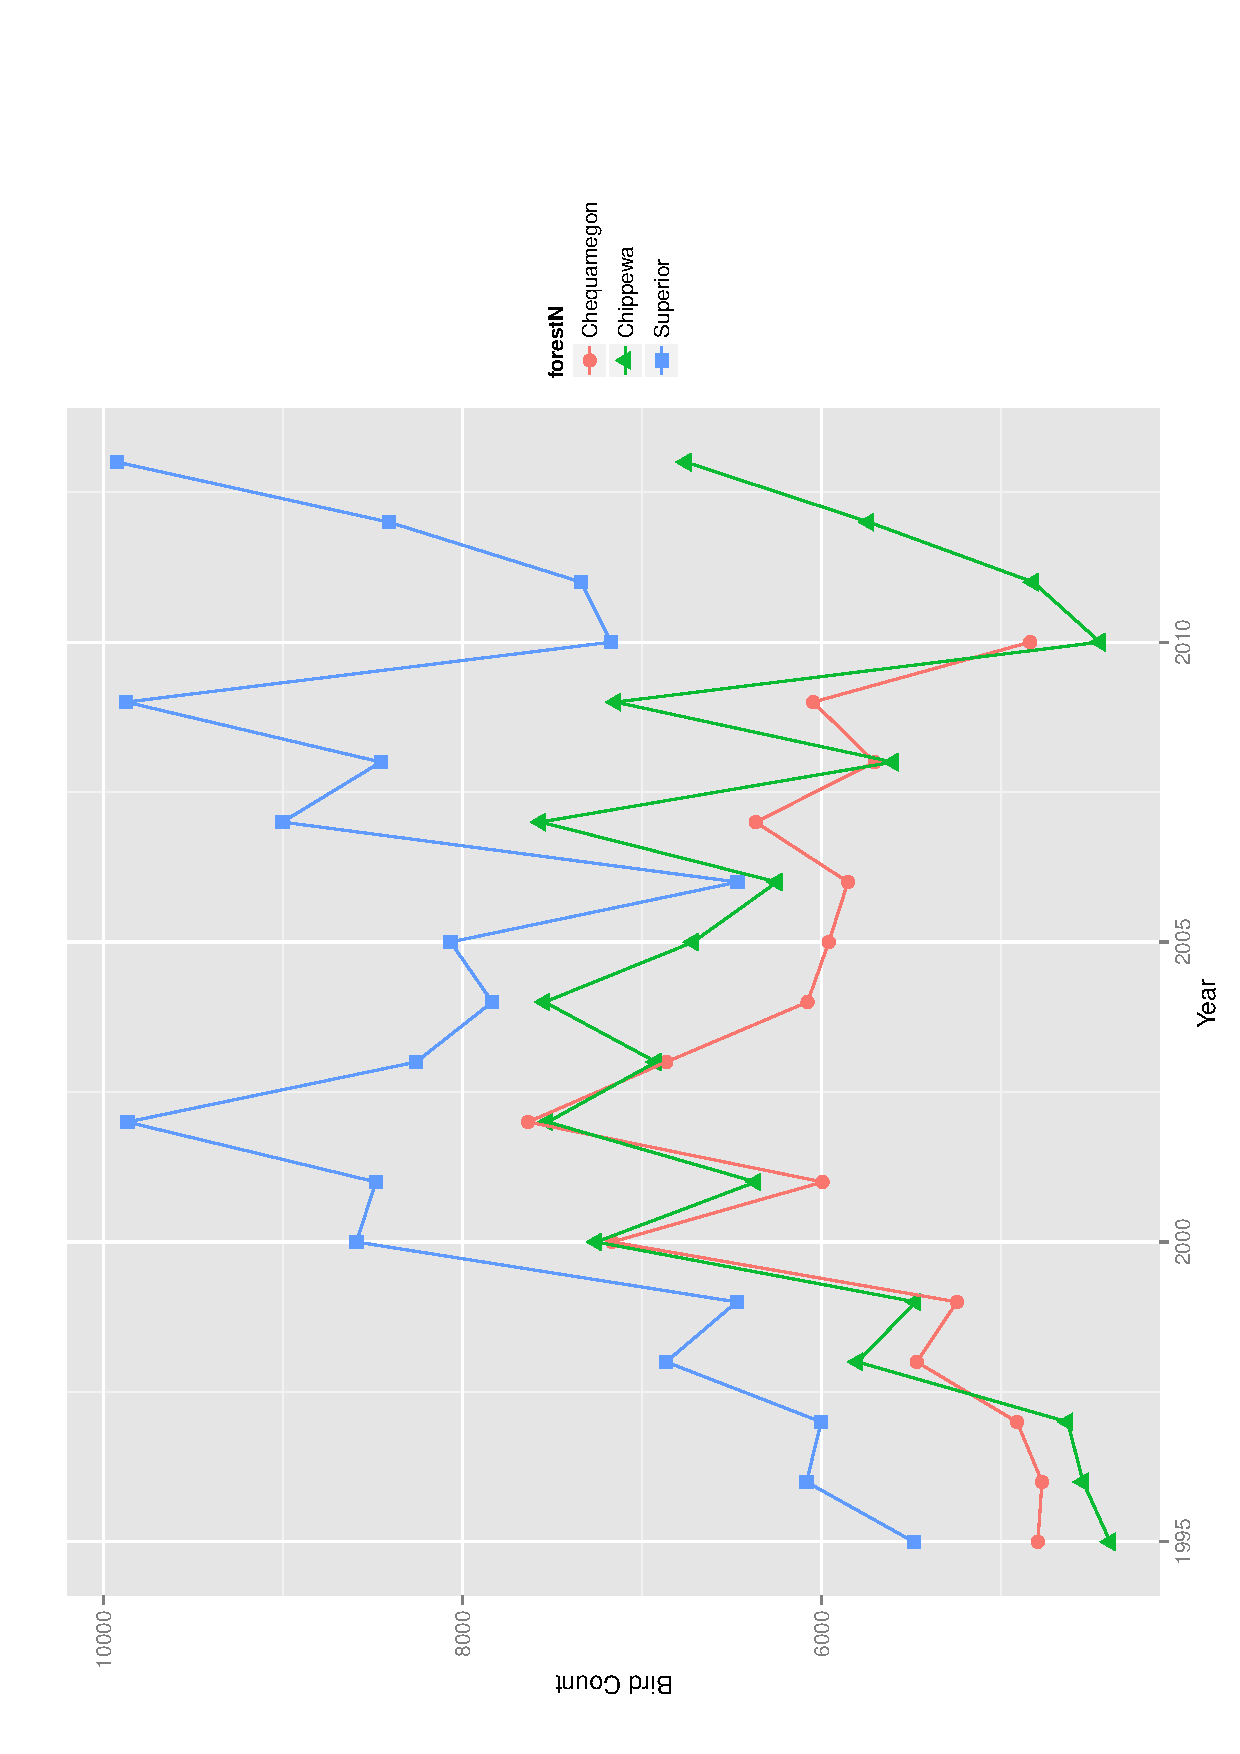
\includegraphics[width =\textwidth]{rawtrend}
 \vspace{-.5in}
\caption{Yearly total birds counts for the 10 selected species \label{figtr} }
\end{figure}

Ovenbirds are consistently the most abundant species over all years in Superior forest,  with more than 1000 bird counts in several occasions. The number of Ovenbird seem to increase until 2002 when they reach its maximum count and decrease since that year, a similar pattern is suggested by the total counts in Chestnut−sided Warbler and Red−eyed Vireo so we expect these species to be positively correlated.  White−throated Sparrow and Nashville Warbler shows an increasing pattern over all the period, and the other species shows a constant patten.  

Table \ref{count07} presents  mean and standard deviation  of the total bird count and the average count for each species, the species are sorted from top to bottom by abundance.  We can appreciate again the differences in total abundances among species. For instance, Ovenbirds are ten times more abundant than the Least Flycatcher. Recall we are selecting the ten most abundant species, which means there are species with really low counts in the entire counting season. 

% latex table generated in R 3.0.2 by xtable 1.7-1 package
% Tue Apr  1 00:13:08 2014
\begin{table}[ht]
\centering
\caption{Total counts on 2007 for the 10 more abundant species} 
\begin{tabular}{llrrr}
  \hline
Specie & Abbrev & Chequamegon & Chippewa & Superior \\ 
  \hline
Least Flycatcher & OVEN & 1003 & 835 & 1168 \\ 
  Blue Jay & REVI & 823 & 997 & 771 \\ 
  White-throated Sparrow & NAWA & 240 & 348 & 867 \\ 
  Red-eyed Vireo & BLJA & 222 & 199 & 230 \\ 
  Nashville Warbler & CSWA & 211 & 330 & 375 \\ 
  Chestnut-sided Warbler & WTSP & 180 & 387 & 940 \\ 
  Ovenbird & HETH & 175 & 249 & 265 \\ 
  Veery & AMRO & 156 & 102 & 154 \\ 
  Hermit Thrush & LEFL & 155 & 368 & 120 \\ 
  American Robin & VEER &  91 & 402 & 264 \\ 
   \hline
\end{tabular}
\end{table}


The information about the abbreviation for the species names is presented in Table \ref{count07} we won't use the common name of the species in the figures and pages that follow we use the abbreviation contained in this table. 

As expected, the sample variances for the total count are much higher than the variances of the mean. This give us the possibility of evaluate the effect of the scaling on the correlations inference, it is not clear that we should model the total count or the mean, so it would be possible to choose any of them. This arbitrary choice however may impact on the posterior inferences about the covariances matrix. 

\subsection{ Correlation among Bird Species}

We want to estimate the species correlation over time, we use information only for Superior forest and for the 10 most abundant species in 2007. This set up for inference similar to the simulated data inference we have already worked with, in this sense we expect the results over real data set will be similar to the ones we observed on simulated data. 

We consider different ``set up'' to estimate the correlation among species, which vary in dimensionality, response variable and covariance matrix prior. In all cases the data will be centered, this might be not realistic but this paper is the covariance matrix and we prefer not considering possible effects of the mean estimation.  

With ten bird species we have 45 correlation coefficients to estimate, the data model is in every case a normal model with zero mean, $Y \sim N_d(0, \Sigma)$, we estimate each correlation several times, using different contexts. 

\begin{description}
\item[Covariance Prior] The main focus of the paper is to understand the effect of  $\Sigma$ prior distribution. Then we consider all the 4 prior distributions described previously, $IW$, $SIW$, $HIW_{ht}$, $BMM_{mu}$ and finally pre-scale data and use the $IW$. 

\item[ Dimensions] The value of $d$ indicate the dimension of the model, we consider two options here. A bivariate case, in which we fit a different model for each pair of species, so this scenario consist in 45 models with 3 parameters each (two variance and the correlation). Also we fit a model for all ten species together, forming one model with 55 parameters (45 correlations and 10 variances). 

\item[Response] We also will use two different response variables. We use the yearly bird count and the yearly average, the latter represent an option with a very little variability in the response while the total count is highly variable. From the simulations results we expect the scale may affect the correlation inference for the $IW$ prior case. 
\end{description}

\begin{figure}[hbpt]
\centering
\includegraphics[width=\textwidth]{rescorr}
 \vspace{-.5in}
\caption{Correlation inference results. Posterior mean for $\rho$  against Pearson correlation coefficient. 
Columns panel represent the dimension of the model (bivariate or ten-dimensional), row panels represent the response variable (average of the count or total count)  and color of the points represent the covariance prior. \label{fig:coring}  }
\end{figure}

\begin{figure}[hbpt]
\centering
\includegraphics[width=\textwidth]{resvar}
 \vspace{-.5in}
\caption{Standard deviation inference results. Scatter-plot of posterior mean for $\sigma_1$  against sample standard deviation. Only for ten dimensional case, columns panel represent response variable (average of the count or total count)  and color of the points represent the covariance prior. \label{birdsd}  }
\end{figure}

Figure \ref{fig:coring} present the estimated correlations, the posterior mean for each model is plotted against the Pearson correlation coefficient. The four panels represent each combination of response and dimension and within each panel there are five estimates for each pair of bird species corresponding to the four priors used. 

These results are quite interesting and match closely with we found on simulated data. When we use the average count as response variable, we see every bayesian estimate is a little bit shrunk towards 0 but the case of the $IW$ this shrinkage is really big. Correlations estimated using IW prior are smaller in absolute value than the rest of the prior options. This effect is expected taking into account that the average count variability is small. 

However results may change if we decide to use a response with high variance as the total count. The $IW$ prior shows a totally different inference picture, now there is no shrunk towards small correlation values and in the case of a ten dimensional model there are several $IW$ correlation median which are actually bigger than Pearson coefficient. 

The $SIW$, $HIW_{ht}$ and $BMM_{mu}$ priors shows similar behavior no matter which is the response used to estimate the covariance matrix, and estimating correlation with any of these priors will lead to basically same conclusions. Finally if we scale the data to have variance equals to 1 then, $IW$ prior shows a similar behavior than the rest.

Inference about standard deviations is presented on figure \ref{birdsd}. Here we present only results for the ten dimensional models, the models using pairs of variables lead to several estimates for the same parameter because each species appears in nine different bivariate models. The standard deviation results also match what we found on simulated data, the only prior showing any problems is $IW$ which overestimate (with respect to the sample standard deviation) standard deviations that are lower than 0.1. 

\begin{figure}[hbpt]
\centering
\includegraphics[width=\textwidth]{corrmat}
 \vspace{-.5in}
\caption{Correlation matrix among ten species used in the study. Using $BMM_{mu}$ prior, average count, and ten dimensional model \label{fig:mat}}
\end{figure}

Figure \ref{fig:mat} present the estimated correlation matrix using an $BMM_{mu}$ prior, on a ten dimensional model and an average count as a response. There were no negative correlated species among the most abundant ones. We can see there are some species forming a sort of a 'cluster" in the series that all are highly correlated, as  OVEN, REVI and CSWA (maybe WTSP could be in this group too).  On the other hand there are a couple of species which shows small correlations with all the rest, this is specially true for LEFL and also AMRO.  

%\begin{figure}[hbpt]
%\centering
%\includegraphics[width=\textwidth]{spcor}
% \vspace{-.5in}
%\caption{Trend in some selected species. OVEN, REVI and CSWA are highly correlated while LEFL and AMRO shows no correlation with other species. \label{trend}}
%\end{figure}
%Figure \ref{trend}  shows the dynamics for the five species identify on the correlation matrix. AS the data are centered, the lines represent the difference between the average yearly count and the historical mean for that species. The three species with high correlation shows the same temporal pattern, a sort of inverted u-shape specially marked on the case of OVEN. The two species with small correlation have a very stable pattern with no big departures from its own mean. 

\section{Discussion} 

We compare several choices for covariance matrix prior, this comparison is based on simulation and visualization tools. 

At a first step, looking at simulations from the prior we see that $IW$ constraint the covariance matrix parameter implying strong dependence among these individual matrix components, correlations tend to be small when variances are small and tends to be high in absolute value when the standard deviation is large, also the variances from different components are positive correlated.  Priors $SIW$ and $HIW_{ht}$ shows similar characteristics than $IW$ but both seem to be more flexible than $IW$ prior. The case of $BMM_{mu}$ is the one presenting the most flexibility since variances and correlations are by construction independent.

In practice what determines the inference for the bayesian model is not the prior but how the posterior looks like. Posterior simulation results for $IW$ prior show this option maintain some the problems we see already in the prior.  The correlation estimate is affected by the scaling of the data, when the variance is low the posterior mean is shrunk towards 0 regardless the true value of the correlation coefficient, but for large values of the variance the correlation seem to be well estimated.  

The other three options for $\Sigma$ prior do not show evident problems capturing the true correlation values for this simulation exercise. Even  $SIW$ and $HIW_{ht}$ who show similar prior characteristic than $IW$ are flexible enough to ensure good results estimating correlations. As we expected $BMM_{mu}$ prior show no big problems estimating  correlation. 

The covariance parameter it well captured by all priors choices, $IW$ present more variability when the standard deviation is low but there is no bias in the covariance estimate. This suggest the reason for underestimating the correlation is precisely the standard deviation overestimation. As the covariance is well estimated, correlation is divided by an overestimated standard deviation and consequently shrunk towards zero. This explains why posterior inference for $IW$ prior shows only problems when the variance is low, since the only standard deviation values that are biased estimated are the small ones. 

\begin{figure}[hbpt]
\centering
\includegraphics[width=\textwidth]{ig}
 \vspace{-.5in}
\caption{Density of $X\sim \mbox{IG}(1, 1/2)$, red line at $x=0.01$. \label{igamma} }
\end{figure}

Figure \ref{igamma} shows the density of an inverse gamma distributed variables for small values. This help us to understand why we observe a bias in the standard deviation using $IW$ prior. The marginal prior distribution for $\sigma_i$ implied by $IW$ prior is $\sigma_i \sim \mbox{IG}(1, 1/2)$ when we set the parameters as $\nu = d+1$ and $\Lambda=I_d$ the usual choice for get non-informative prior. The red line is drawn at 0.01 value where the prior put no probability mass which explains the overestimation we have observe on simulation study and with the bird count data. 


The main question that arise at this point is: What prior should we use ? 

From a modeler point of view, the $BMM_{mu}$ prior flexibility is appealing since we can model correlations and variance in separate fashion and will be the data what define its relationship.  This way so set up a separation strategy is the original proposal of \cite{barnard2000}, however a separation strategy could use any other prior, for instance a half-t or uniform which are better within the hierarchical models context.  From a computational perspective we expect the $BMM_{mu}$ prior the most complex, since all the others conserve the conjugacy properties of the $IW$ distribution This is specially relevant for a Gibbs sampler, where conjugacy allow to get a full Gibbs step instead a metropolis one, Using Stan software which is base in Hamiltonian Monte Carlo strategy to obtain samples from posterior there is no that much cost to paid for using a non conjugate prior as the $BMM_{mu}$.  Results for $SIW$ prior show much better computational performance than the rest with the best ratio between effective sample size over time.  

In summary, the answer to the previous question may depend on which are the computational resources we are working with 

\begin{itemize}
\item  if it is possible to use a HMC sampler as STAN the separation strategy proposed by \cite{barnard2000} gives modeling flexibility and good inferences properties. But computational performance is poor, this should be improve in order to use this strategy as the general default option. Maybe sampling directly from the correlation matrix distribution is the way to improve its computational performance.  

\item Whenever we use Gibbs base samplers (as JAGS or BUGS) a prior which maintain conjugacy might be preferable such as the scaled inverse Wishart. This prior shown good computational performance and nice inference properties.  

\item For some models the samplers does not allow to fit these priors and we are constraint to use the classical inverse Wishart distribution. In this case, we may recommend to scale the data by dividing each variable for the sample standard deviation. This way we can avoid possible biased estimates for standard deviations and correlations. 
\end{itemize}

There are multiple ways in which we could continue with this line of work. However, there are three issues that seems more natural ways to continue. 

\begin{description} 
\item[Different Model] We want to extend this study into the context to hierarchical models where the covariance matrix prior is not for the data model but for modeling a set of coefficient in a linear predictor. \cite{gelman2006prior} suggest the effect of prior distributions on variance parameters is different when these parameters appear in the data model and when appears as an hyper-parameter in the model. So it will be interesting to evaluate if what we see on this simulation study can be extended to a linear model context. This would be also the case where a re-scaling of data solution for the $IW$ has different meaning. It is possible to fit the model twice, one for estimate the appropriate scaling parameter and a second one to estimate the covariance matrix, however we should take into account the variability in the first stage of estimation. 

\item[Different Scenarios]  Here we use for simulations covariance matrices with all variances and all correlations to be equal. What happen when there is one large variance and one very low ? It might be possible that if the larger one is large enough to reduce the bias in the correlation when we use $IW$ prior. 

\item[Different Priors]A deeper study on priors for correlation matrices as the LKJ prior could give better ways to implement a separation strategy. This would likely improve the computational performance of the separation strategy compared with $BMM_{mu}$, since LKJ prior is already a Stan function. If we could find the way to set the LKJ parameter value to ensure marginally uniform correlations this strategy would be really appealing. 
\end{description}


\bibliographystyle{asa}      
\bibliography{report_year}      

\appendix
\section{Appendix}

\begin{figure}[hbpt]
   \centering
   \includegraphics[width=\textwidth]{fig_rho_d10} % requires the graphicx package
    \vspace{-.5in}
   \caption{ Ten-dimensional data results. Scatter-plot of posterior mean for $\rho$  against correlation true value used in simulation. Each panel is a combination of standard deviation (columns) and sample size (rows),  color and shape of the points represent the covariance prior. \label{rhod10} }
\end{figure}

\begin{figure}[hbpt]
   \centering
   \includegraphics[width=\textwidth]{fig_d2d10} % requires the graphicx package
    \vspace{-.5in}
   \caption{ Comparison between two dimensions options. Posterior mean for $\rho$ within the ten-dimensional data against posterior mean of $\rho$ within the bivariate data. Each panel is a combination of standard deviation (columns) and sample size (rows),  color and shape of the points represent the covariance prior.\label{d2d10} }
\end{figure}

\begin{figure}[htbp]
   \centering
   \includegraphics[width=\textwidth]{fig_s1_d10} 
    \vspace{-.5in}
   \caption{Ten-dimensional data results. Scatter-plot of posterior mean for $\sigma_1$  against standard deviation true value used in simulation. Each panel is a combination of correlation (columns) and sample size (rows),  color and shape of the points represent the covariance prior.  \label{devF2} }
\end{figure}
\end{document}


%============================================================================================
%% 	LINEAR MODEL STUFF MOVE OUT OF THE REPORT 


%\subsection{Hierarchical Linear Models}

%Usually the multivariate normal distribution does not appear directly to model data, the common models assumes independence along observations and when this assumption it is not present the covariance matrix is modeled with a specific structure such as compound cemetery in a random effects model. 

%Instead multivariate normal model is a very commonly used as a distribution of a linear model coefficients within the context of a hierarchical model. Le assume we are interested in a model like  $Y_s \sim N(X_s\beta_s, \sigma_s)$ where the subscript $s$ is representing the different groups in the model. 
%In the concrete data set, we use time as the main covariate variable and a response variable changing over time, also the data are grouped according bird, then $Y_{ts}$ will be related to the average bird count for group $s$ at time $t$ and an model example could be $Y_ts \sim N(\beta_{1s} + t\beta_{2s}, \sigma_s)$. 
%
%In order to make inference from this modle within a bayesian framework, we need to decide priors for $(\beta_s, \sigma_s)$ parameters. One key decision for this choice is how to combine information across groups. We may want to set a separate prior for each parameter within each group, making each group model completely independent from the rest. On the opposite side we could combine all the groups into one set of parameters $(\beta_s, \sigma_s) = (\beta, \sigma)$. Finally as a compromise between the previous options we can allows different parameters for each group but all with common prior distribution, i.e. a hierarchical model. 
%
%These options on how combine information across groups can be done independently for $\beta_s$ and $\sigma_s$, which lead us to a nine ways setting up the prior distributions for all the parameters in the model. Table \ref{stmod} presents the basic choices of models we just described, rows of the table are the three ways we can combine the groups information for the $\beta_s$ coefficients and the columns represents the same thing but for $\sigma_s$ instead. The result are nine models, each of the nine cells in Table \ref{stmod} represents one of those combination. 
% 
%\begin{table}[h]
%\caption{Basic Prior Structure Choices. In all cases the data model consist in a multivariate regression $Y_s \sim N(X_s\beta_s,\sigma_s^2)$, also in all models the prior for the vector $\beta_s$ is a normal distribution, $N(\mu, \Sigma)$ but  parameters $\mu$ and $\Sigma$ might be learned from the data or set as a fixed value. \label{stmod} } 
%\begin{tabular}{|l|ccc|} \hline \hline
%& Same $\sigma$s ($\sigma_s=\sigma$) & Hierarchical $\sigma$s & Different $\sigma$s \\ \hline\hline
%Same   
%%&$Y_s \sim N(X_s\beta,\sigma^2)$&$Y_s \sim N(X_s\beta,\sigma_s^2)$& $Y_s \sim N(X_s\beta, \sigma_s^2)$ \\
%$\beta$s &$\mu=\mu_0, \Sigma=\Sigma_0$ &$\mu=\mu_0, \Sigma=\Sigma_0$&$\mu=\mu_0, \Sigma=\Sigma_0$ \\
%($\beta_s = \beta$ ) & $\sigma\sim unif(0, v_0)$ &$\sigma^2_s\sim IG(\alpha_s/2, \alpha_s\lambda_s/2)$& $\sigma_s\sim unif(0, v_0)$ \\ 
%& & $\alpha_s \sim unif(0,a_0)$ & \\ 
%& & $\lambda_s\sim unif(0,l_0)$ & \\ \hline 
%hierarchical $\beta$s
%%&$Y_s \sim N(X_s\beta,\sigma^2)$&$Y_s \sim N(X_s\beta,\sigma_s^2)$& $Y_s \sim N(X_s\beta, \sigma_s^2)$ \\
%%&$\beta_s\sim N(\mu, \Sigma)$&$\beta_s\sim N(\mu, \Sigma)$ & $\beta_s\sim N(\mu,\Sigma)$ \\
%& $\mu \sim N(\psi_0, \Psi_0) $ & $\mu \sim N(\psi_0, \Psi_0) $ & $\mu \sim N(\psi_0, \Psi_0) $ \\ 
%& $\Sigma \sim IW(R_0,d_0)$& $\Sigma \sim IW(R_0,d_0)$& $\Sigma \sim IW(R_0,d_0)$ \\  
%&$\sigma\sim unif(0, v_0)$ &$\sigma^2_s\sim IG(\alpha_s/2, \alpha_s\lambda_s/2)$& $\sigma_s\sim unif(0, v_0)$ \\ 
%& & $\alpha_s \sim unif(0,a_0)$& \\
%& & $\lambda_s\sim unif(0,l_0)$ & \\ \hline 
%different $\beta$s
%%&$Y_s \sim N(X_s\beta,\sigma^2)$&$Y_s \sim N(X_s\beta,\sigma_s^2)$& $Y_s \sim N(X_s\beta, \sigma_s^2)$ \\
%%&$\beta_s\sim N(\mu_0, \Sigma_0)$&$\beta_s\sim N(\mu_0, \Sigma_0)$&$\beta_s\sim N(\mu_0, \Sigma_0)$ \\
%&$\mu=\mu_0, \Sigma=\Sigma_0$ &$\mu=\mu_0, \Sigma=\Sigma_0$&$\mu=\mu_0, \Sigma=\Sigma_0$ \\
%&$\sigma\sim unif(0, v_0)$ &$\sigma^2_s\sim IG(\alpha_s/2, \alpha_s\lambda_s/2)$& $\sigma_s\sim unif(0, v_0)$ \\ 
%& & $\alpha_s \sim unif(0,a_0)$ & \\
%& & $\lambda_s\sim unif(0,l_0)$ & \\ \hline\hline
%\end{tabular} \\
%\tiny{Every letter with subscript 0 represent a numeric value and is not learned from data, $IW$ represents an inverse Wishart distribution and $IG$ an inverse gamma distribution.}
%\end{table}
%
%Some comments about the models and notation contain in Table \ref{stmod}. 
%First, all the symbols with ''0'' subscript represent numerical known values not parameters we learn from data. Usually these parameter are set to assure the non informativity of the prior. For instance $v_0$, $a_0$ and $l_0$ are the upper limits of uniforms distributions for variance parameter or hyperparameter and then will be set as very high numerical values. 
%
%Second, every model is written in matrix form. Vector $Y_s$ represent all observations for group $s$, $Y_s =  (Y_{s1},Y_{s2},\dots,Y_{sn})^{'}$, in same way $X_s$ is a $n \times k$ matrix containing the observed values for $k$ predictor variables. 
%Accordingly, parameters are also in matrix form, so $\beta_s$ and $\mu$ are $k$-dimensional vectors representing each predictor effect for the group $s$ and its prior mean, while $\Sigma$ is the $k\times k$ covariance matrix for $\beta_s$ (note that $\mu_0$ and $\Sigma_0$ are numerical values not parameters, so they are not vector or matrices just scalar known values). 
%
%Third, in every case the deepest layer in the model is some uniform distribution for a variance parameter or for a variance hyper-parameter. We choose a uniform prior on standard deviation scale for $\sigma_s$ and its related hyperparameters, this is following Gelman recommendation on REF, but we could set a different options as inverse gamma flat prior as recomended on REF or an improper prior. 
%
%As examples, we describe the three models that lies in the diagonal of the table \ref{stmod}. 
%
%The first model consist in a situation where we are ignoring the existence of different group and just estimating one set of $\beta$ and one value of $\sigma$ so this is actually one regression on the entire data. On the other hand, the ''last'' cell in the table (column 3, row 3) is representing a separate regressions for each group with flat priors on all parameters. In this case the $\Sigma_0$ matrix is a diagonal matrix
%
%Finally, the central cell model represent a fully hierarchical model in both $\sigma$ and $\beta$. The covariance matrix $\Sigma$ is learned form data, so we want to model the dependency across the linear predictor coefficient.  Here the choice of $p(\Sigma)$ is really important, ''it determines the nature of the shrinkage of the posterior of the individual $\beta_j$ towards a common target'' (\cite{barnard2000}). 
%What is the effect of the covariance matrix prior on the inference about the linear model coefficients ?  This is an important question we would like to address. 



%\subsection{ Bird Populations trends} 
%According to (REF, Etterson) one of the basic research goals in Ecology consist on understand the distribution and abundance of the animal population. In this work, the particular goal will be to explore alternatives to model the time trends in Western Great Lakes Birds population over 1994 to 2011. As a starting point we consider separate regression equations for each specie and forest, a model for one species is represented on equation \ref{mod1}. 
%\begin{eqnarray}
%\nonumber Y_{ts} &=&  \beta_{0s} + \beta_{1s}t + \beta_{2s}t^2 + \epsilon_{ts}  \\
%\epsilon_{ts} &\sim& N(0,\sigma_{s}^2)
%\label{mod1}
%\end{eqnarray}
%where $Y_{ts}$ represent the average bird count on year $t$ in the forest $f$ for the specie $s$. From a bayesian point of view this consist in a hierarchical Normal model where $Y_{ts}\vert (\beta_{0s},\beta_{1s},\beta_{2s},\sigma_{s}) \sim N(\beta_{0s}+\beta_{1s}t+\beta_{2s}t^2, \sigma_{s})$ and all parameters are independents with flat priors and different values for each species. 
%
%There are 73 species and we fit the model \ref{mod1} for 3 different forests there are 219 individual species regression models in total. In addition, we consider two variants from \ref{mod1}. First, it is not clear that we need to include a quadratic term in the regression term so we may consider a simple regresion only. Second, it is common to log transform the average counts. So, for each species we consider 4 models including two types of response variable (in logs and average count) and two set of predictors (quadratic and only linear). 
% 
%Along this report the parameters of interest will be the regression slope for each species.  Figure \ref{histm1} presents these slopes median for each species on every scenario we run for all three forest. There are 12 panels, each row represent one forest (Chequamegon, Chippewa and Superior) and each column represent one type of model (linear in logs, quadratic in logs, linear with counts and quadratic with counts).  
%\begin{figure}[h!]
%\centering
%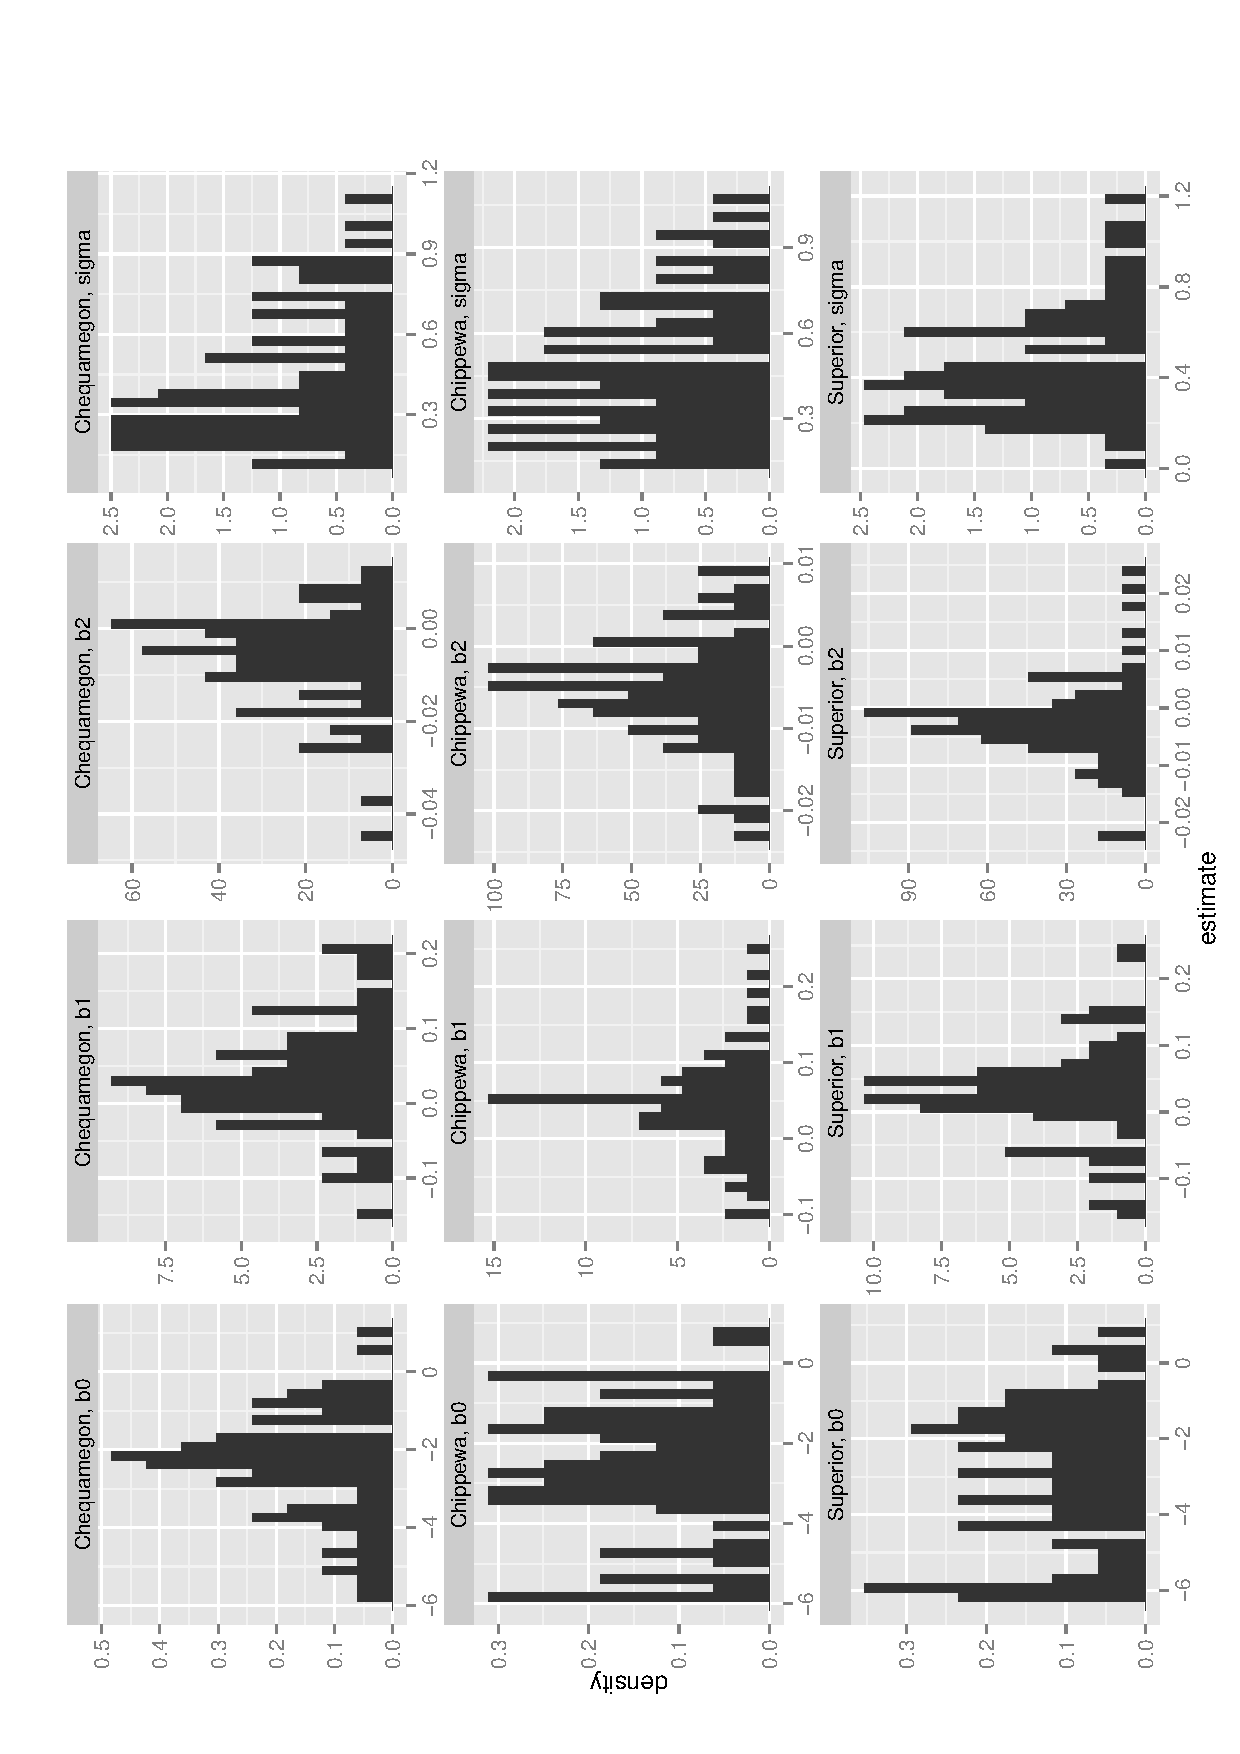
\includegraphics[scale=.5]{hist_m1}
%\caption{Species slopes from model \ref{mod1} . \label{histm1}}
%\end{figure}
%
%The slopes histograms are similar on the 3 forest within each model type. The model with the log transformed response seem to present a more symmetric distribution of the slopes, when we use the average counts most of the slopes are very close to zero value except for a few species with high slope values. 
%
%Next, we explore the bivariate relation among the coefficients within each regression. With this in mind we can see a scatter matrix of the estimated coefficients in Figure \ref{pairss1}. The main point to see here is a negative relation between the slope and the quadratic term for all forest, is .67, .82 and .83 on Chequamegon, Chippewa and Superior respectively. (KAISER Dix it: while polynomials are wonderfully flexible functions for describing data patterns, they do not lend themselves to interpretation of coefficient values -different combinations of constant, linear, and quadratic terms can lead to quite similar functions over a finite range of covariate values) 
%
%\begin{figure}[h!]
%\centering
%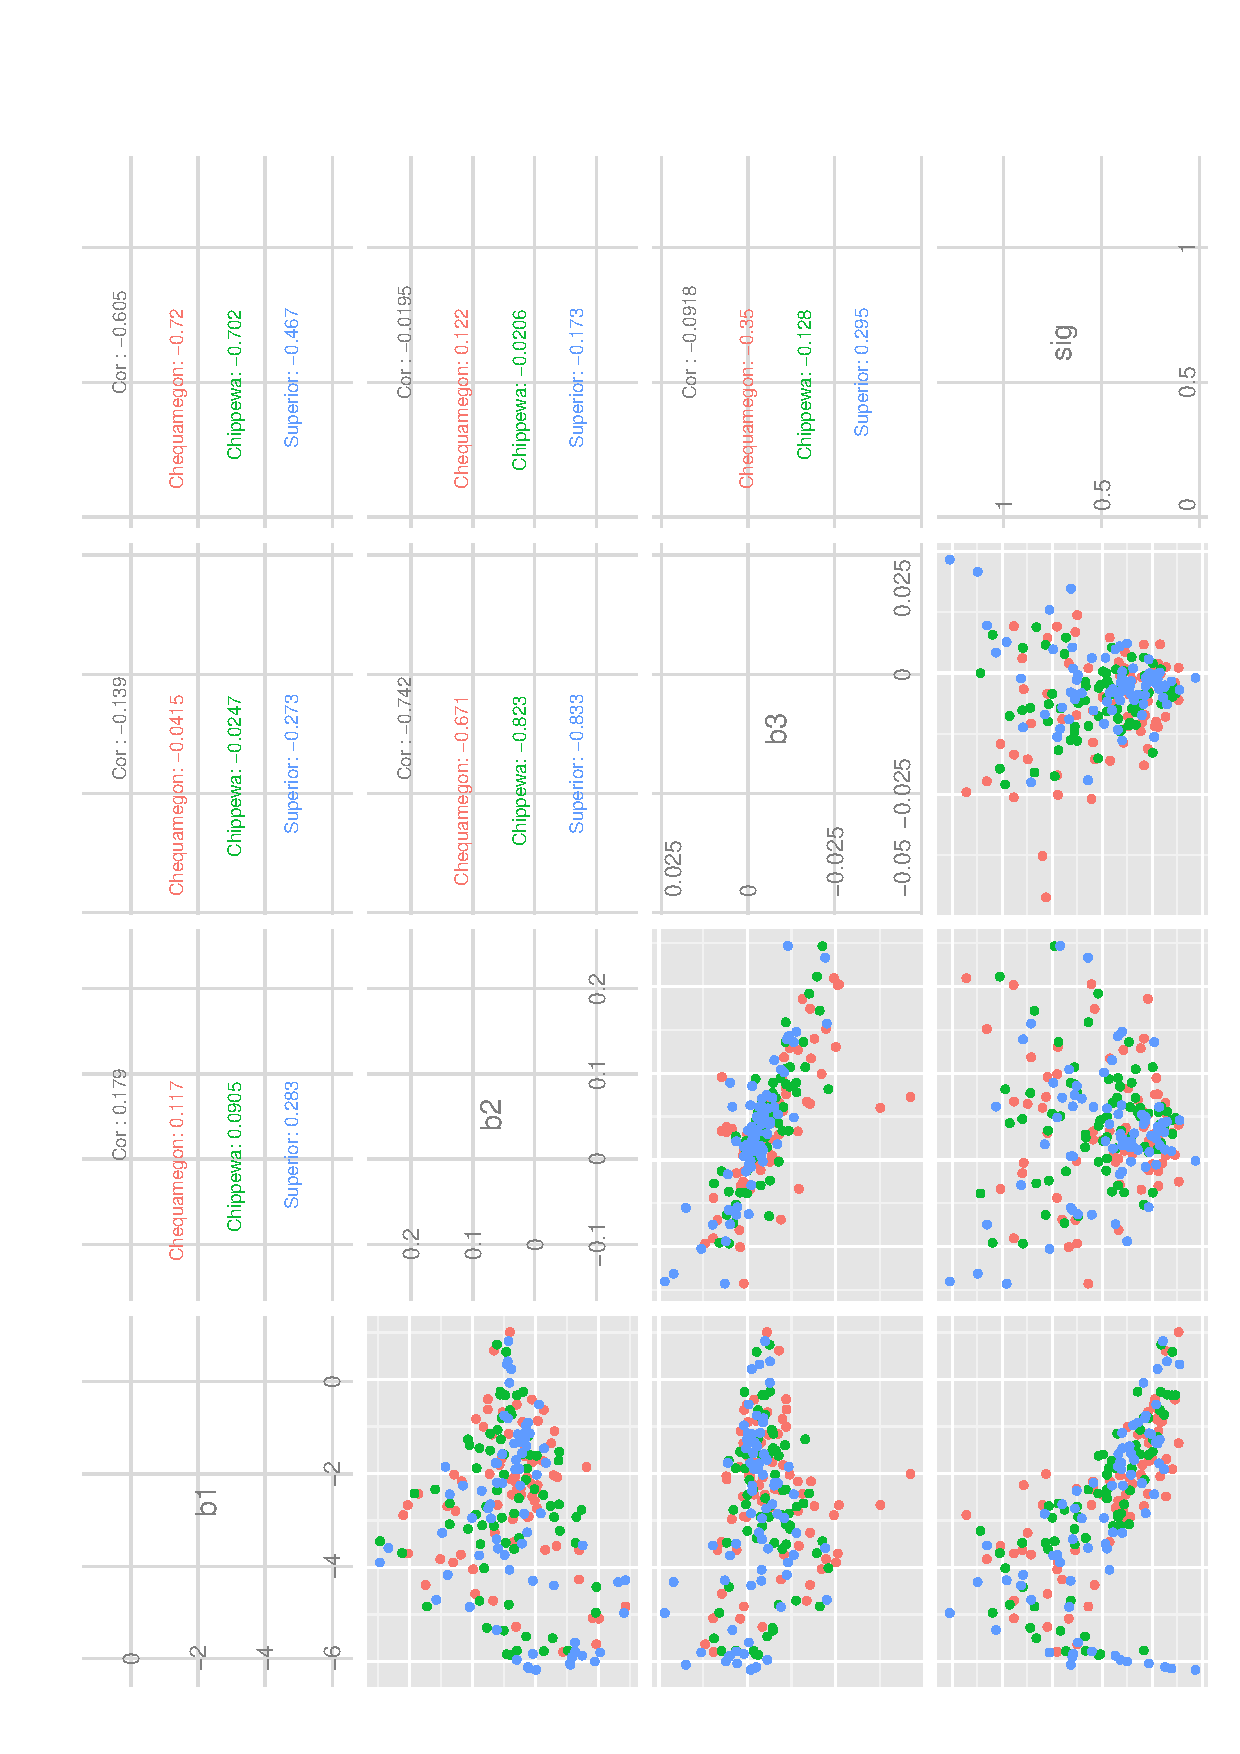
\includegraphics[scale=.6]{scat_m1}
%\caption{Bivariate relation among coefficients of model \ref{mod1}. \label{pairs1}}
%\end{figure}
%Also, there is a negative relation between between intercept and variance, specially for Chequamegon and Chippewa forest. Maybe the main message for this plot is that we should not treat this parameters as independent and try to include their dependence into the model we are fitting. 
%\begin{figure}[h!]
%\centering
%\includegraphics[height=12cm, width=5cm, angle=-90]{gelman.ps}
%\caption{Multivariate Gelman Diag statistic for all models. \label{gel1}}
%\end{figure}
%
%\begin{figure}[h!]
%\centering
%\includegraphics[scale=.6, angle=-90]{slp_bet.ps}
%\caption{ Slope estimates within each type of variance model}
%\end{figure} 
%
%\begin{figure}[h!]
%\centering
%\includegraphics[scale=.6, angle=-90]{rates.ps}
%\caption{ Change Rates within each type of variance model}
%\end{figure} 
%
%\begin{figure}[h!]
%\centering
%\includegraphics[scale=.6, angle=-90]{var_hhll.ps}
%\caption{$Sigma$ posterior distribution visualization plot}
%\end{figure} 
%
%\begin{figure}[h!]
%\centering
%\includegraphics[scale=.6, angle=-90]{var_hhql.ps}
%\caption{$Sigma$ posterior distribution visualization plot}
%\end{figure} 
%%%%%%%%%%%%%%%%%%%%%%%%%%%%%%%%%%%%%%%%%%%%%%%%%%%%%%%%%%%%%%%%%%%%%%%%
